%%%%%%%%%%%%%%%%%%% vorlage.tex %%%%%%%%%%%%%%%%%%%%%%%%%%%%%
%
% Beispiel-Vorlage zur Erstellung von Projekt-Dokumentationen
%
% Benutzen Sie bitte diese Datei um Ihre Dokumente zu erstellen
%
%%%%%% erstellt anhand svmono-Springer-Verlag-Vorlage %%%%%%%%%


%%%%%%%%%%%%%%%%%%%%%%%%%%%%%%%%%%%%%%%%%%%%%%%%%%%
\documentclass[envcountsame,envcountchap, deutsch]{i-studis}


\usepackage{makeidx}         % Erlaubt die Erzeugung eines Index-Verzeichnisses
\usepackage{multicol}        % Zweispaltiger Index-Verzeichnis
%\usepackage[bottom]{footmisc} % Erzeugung von Fu�noten nur beim Bedarf einbinden

%%-----------------------------------------------------
%\newif\ifpdf
%\ifx\pdfoutput\undefined
%\pdffalse
%\else
%\pdfoutput=1
%\pdftrue
%\fi
%%--------------------------------------------------------
%\ifpdf
\usepackage[pdftex]{graphicx}
\usepackage[pdftex,plainpages=false]{hyperref}
%\else
%\usepackage{graphicx}
%\usepackage[plainpages=false]{hyperref}
%\fi
%%-----------------------------------------------------
\usepackage{color}	% Farbverwaltung
%\usepackage{ngerman} % Neue deutsche Rechtsschreibung
\usepackage[english, ngerman]{babel}
\usepackage[latin1]{inputenc} % Erm�glicht Umlaute-Darstellung
%\usepackage[utf8]{inputenc}  % Ermöglicht Umlaute-Darstellung unter Linux (je nach verwendetem Format)
%-----------------------------------------------------
\usepackage{listings} % Code-Darstellung
\lstset
{% general command to set parameter(s)
	basicstyle=\scriptsize, % print whole listing small
	keywordstyle=\color{blue}\bfseries,
	% underlined bold black keywords
	identifierstyle=, % nothing happens
	commentstyle=\color{red}, % white comments
	stringstyle=\ttfamily, % typewriter type for strings
	showstringspaces=false, % no special string spaces
	framexleftmargin=7mm, 
	tabsize=3,
	showtabs=false,
	frame=single, 
	rulesepcolor=\color{blue},
	numbers=left,
	linewidth=146mm,
	xleftmargin=8mm
}
\usepackage{textcomp} % celsius - Darstellung
\usepackage{
amssymb,
amsfonts,
amstext,
amsmath
} % Mathematische Symbole
\usepackage[german, ruled, vlined]{algorithm2e}
\usepackage[a4paper]{geometry} %Andere Formatierung
\usepackage{bibgerm}
\usepackage{array}
\hyphenation{Ele-men-tar-ob-jek-te  ab-ge-tas-tet Aus-wer-tung House-holder-Matrix Le-ast-Squa-res-Al-go-ri-th-men} %Silbentrennung bei falschen Trennung angeben
\setlength{\textheight}{1.1\textheight}
\pagestyle{myheadings} % Erzeugt selbstdefinierte Kopfzeile
\makeindex % Index-Erstellung

% Ab hier beginnt das eigentliche Dokument.
%--------------------------------------------------------------------------
\begin{document}

%------------------------- Titelblatt -------------------------------------
\title{Titel der Projekt- Abschlussarbeit auf Deutsch}
\subtitle{English Title of Project Work}
%---- Die Art der Dokumentation kann hier ausgew�hlt werden---------------
%\project{Master Abschlussarbeit}
%\project{Master Projektstudium}
%\project{Bachelor Abschlussarbeit}
%\project{Projektarbeit}
%\project{Seminar zur Vorlesung ...}
\project{Hausarbeit zur Vorlesung ...}
%--------------------------------------------------------------------------
\supervisor{Titel Vorname Name} % Betreuer der Arbeit
\author{Autor} %Autor der Arbeit
\address{Ort,} % Im Zusammenhang mit dem Datum wird hinter dem Ort ein Komma angegeben
\submitdate{Abgabedatum} % Abgabedatum
%\begingroup
%  \renewcommand{\thepage}{title}
%  \mytitlepage
%  \newpage
%\endgroup
\begingroup
  \renewcommand{\thepage}{Titel}
  \mytitlepage
  \newpage
\endgroup
%--------------------------------------------------------------------------
\frontmatter 
%--------------------------------------------------------------------------
%\danksagung

Dank an ... %Danksagungen
%\preface

Ein Vorwort ist nicht unbedingt n�tig. Falls Sie ein Vorwort schreiben, so ist dies der Platz, um z.B. die
Firma vorzustellen, in der diese Arbeit entstanden ist, oder einigen Leuten zu danken, die in irgendeiner
Form positiv zur Entstehung dieser Arbeit beigetragen haben. Auf keinen Fall sollten Sie im Vorwort die
Aufgabenstellung n�her erl�utern oder vertieft auf technische Sachverhalte eingehen.
%%%%%%%%%%%%%%%%%%%%%%% Kurzfassung.tex %%%%%%%%%%%%%%%%%%%%%%%%%%%%%%%%%%%%%
%
% sample preface
%
% Use this file as a template for your own input.
%
%%%%%%%%%%%%%%%%%%%%%%%% Springer-Verlag %%%%%%%%%%%%%%%%%%%%%%%%%%

\kurzfassung

%% Schreiben Sie Ihre Kurzfassung hierher
Hier soll eine Kurzfassung der Arbeit stehen. Eine halbe Seite sollte gen�gen. Die Kurzfassung gibt
in einer verst�ndlichen Form den Gegenstand und das Ergebnis der Arbeit an. Sie soll dem Leser
vermitteln, um was es geht und was die Leistung der Arbeit ist. Damit kann der Leser entscheiden,
ob Thema, Inhalt und Ergebnis der Arbeit f�r so ihn interessant sind, dass er sie liest.
\\[3ex]

%% Please write your preface here
\noindent
The same in english (option).

 % Kurzfassung Deutsch/English
\tableofcontents %Inhaltsverzeichnis - notwendig
\listoffigures % Abbildungsverzeichnis - optional
\listoftables % Tabellenverzeichnis- optional
%--------------------------------------------------------------------------
\mainmatter                        %Hauptteil (ab hier arab. Seitenzahlen)
%--------------------------------------------------------------------------
% Kapitell werden einzeln abgespeichert und hier eingef�gt
%\chapter{Einleitung}
Begonnen werden soll mit einer Einleitung zum Thema: z.B. Hintergrund und Ziel
(was, warum).

%\chapter{Problemstellung}

Hier wird i.d.R. zun�chst das generell vorliegende Problem diskutiert: Was ist zu l�sen - was gibt
es bisher an L�sungsans�tzen (prinzipiell) und warum ist es wichtig, dass man dieses Problem l�st.
Letzteres ergibt sich oftmals aus der vorliegenden Anwendungssituation: Man braucht die L�sung, um
eine bestimmte Aufgabe zu erledigen, ein System aufzubauen etc. Der Bezug auf vorhandene oder auch
bisher fehlende L�sungen begr�ndet auch die Intension und Bedeutung dieser Arbeit. Dies k�nnen
allgemeine Gesichtspunkte sein - man liefert einen Beitrag f�r ein generell erkanntes oder zu
erkennendes Problem - oder man hat eben eine spezielle Systemumgebung oder Produkt (z.B. in einer
Firma u.s.w.), woraus sich dieses noch zu l�sende Problem ergibt.

Die genaue Problematik und Randbedingungen werden dann in Kapitel \hyperref[Aufgabenstellung]{Kapitel~\ref{Aufgabenstellung}}
dargestellt.
%\chapter{Aufgabenstellung und Zielsetzung}\label{Aufgabenstellung}

Hier wird nun die Aufgabenstellung konkret dargestellt: Was ist spezifisch zu l�sen? Welche
Randbedingungen sind prinzipiell gegeben und was ist die Zielsetzung? Letztere soll das
beschreiben, was man mit dieser Arbeit (mindestens) erreichen m�chte.
%\chapter{�brige Abschnitte (Kapitel und Abs�tze)}
Die Gliederung h�ngt nat�rlich vom Thema und von der L�sungsstrategie ab. Als n�tzliche
Anhaltspunkte k�nnen die Entwicklungsstufen oder - schritte z.B. der Softwareentwicklung betrachtet
werden. N�tzliche Gesichtspunkte erh�lt und erkennt man, wenn man sich
\begin{itemize}
  \item in die Rolle des Lesers oder
  \item in die Rolle des Entwicklers, der die Arbeit z.B. fortsetzen, erg�nzen oder pflegen soll,
\end{itemize}
versetzt. In der Regel wird vorausgesetzt, dass die Leser einen fachlichen Hintergrund haben - z.B.
Informatik studiert haben. D.h. nur in besonderen, abgesprochenen F�llen schreibt man in popul�rer
Sprache, so dass auch Nicht-Fachleute die Ausarbeitung prinzipiell lesen und verstehen k�nnen.

Die �u�ere Gestaltung der Ausarbeitung hinsichtlich Abschnittformate, Abbildungen, mathematische
Formeln usw. wird in \hyperref[Stile]{Kapitel~\ref*{Stile}} kurz dargestellt.
%\chapter{Latex-Bausteine}\label{Stile}

Der Text wird in bis zu drei Ebenen gegliedert:

\begin{enumerate}
  \item Kapitel ( \verb \chapter{Kapitel} ), \index{Kapitel}
  \item Unterkapitel  ( \verb \section{Abschnitt} ) und
  \item Unterunterkapitel  ( \verb \subsection{Unterabschnitte} ).
\end{enumerate}

\section{Abschnitt}\index{Abschnitt}
Text der Gliederungsebene 2.


\subsection{Unterabschnitt} \index{Unterabschnitt}
Text der Gliederungsebene 3.
Text Text Text Text Text Text Text Text Text Text Text Text Text Text Text
Beispiel f�r Quelltext\index{Quelltext} \\[2 ex]
\noindent
\begin{minipage}{1.0\textwidth} \small
\begin{lstlisting}
	Prozess 1:
	
	Acquire();
		a := 1;
	Release();
	...
	Acquire();
	if(b == 0)
	{					
		c := 3;
		d := a;
	}				
	Release();
\end{lstlisting}
\end{minipage}

\vspace{2cm}
\noindent
\begin{minipage}{1.0\textwidth} \small
\begin{lstlisting}
	Prozess 2:
	
	Acquire();
		b := 1;
	Release();
	...
	Acquire();
	if(a == 0)
	{					
		c := 5;
		d := b;
	}				
	Release();
\end{lstlisting}
\end{minipage}
\vskip 1em

Gr��ere Code-Fragmente sollten im Anhang eingef�gt werden.

\section{Abbildungen und Tabellen}

Abbildung\index{Abbildung} und Tabellen\index{Tabelle} werden zentriert eingef�gt. Grunds�tzlich sollen sie
erst dann erscheinen, nach dem sie im Text angesprochen wurden (siehe Abb. \ref{a1}). Abbildungen und Tabellen (siehe Tabelle \ref{t1}) k�nnen
im (flie�enden) Text (\verb here ), am Seitenanfang (\verb top ), am Seitenende
(\verb bottom ) oder auch gesammelt auf einer nachfolgenden Seite (\verb page )
oder auch ganz am Ende der Ausarbeitung erscheinen. Letzteres sollte man nur
dann w�hlen, wenn die Bilder g�nstig zusammen zu betrachten sind und die
Ausarbeitung nicht zu lang ist ($< 20$ Seiten).

\begin{figure} %[hbtp]
	\centering
		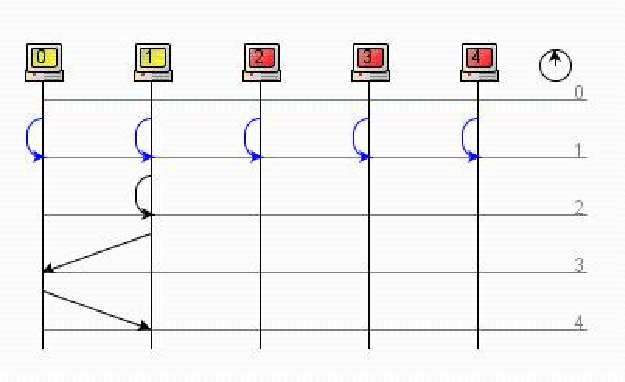
\includegraphics{images/p1ReadSeq.pdf}
	\caption{Bezeichnung der Abbildung}
	\label{a1}
\end{figure}

\begin{table} %[hbtp]
	\centering
		\begin{tabular}{l | l l l l}
		\textbf{Prozesse} & \textbf{Zeit} $\rightarrow$ \\
		\hline
			$P_{1}$ & $W(x)1$ \\
			$P_{2}$ & & $W(x)2$ \\
			$P_{3}$ & & $R(x)2$ & & $R(x)1$\\
			$P_{4}$ & & & $R(x)2$ & $R(x)1$\\
		\end{tabular}
	\caption{Bezeichnung der Tabelle}
	\label{t1}
\end{table}


\section{Mathematische Formel}\index{Formel}
Mathematische Formeln bzw. Formulierungen k�nnen sowohl im
laufenden Text (z.B. $y=x^2$) oder abgesetzt und zentriert im Text
erscheinen. Gleichungen sollten f�r Referenzierungen nummeriert
werden (siehe Formel \ref{gl-1}).
\begin{equation}
\label{gl-1}
e_{i}=\sum _{i=1}^{n}w_{i}x_{i}
\end{equation}

Entscheidungsformel:

\begin{equation}
\psi(t)=\left\{\begin{array}{ccc}
1 &  \qquad 0 <= t < \frac{1}{2} \\
-1 &  \qquad \frac{1}{2} <= t <1 \\
0 & \qquad sonst
\end{array} \right.
\end{equation}


Matrix:\index{Matrix}
\begin{equation}
A = \left(
\begin{array}{llll}
a_{11} & a_{12} & \ldots & a_{1n} \\
a_{21} & a_{22} & \ldots & a_{2n} \\
\vdots & \vdots & \ddots & \vdots \\
a_{n1} & a_{n2} & \ldots & a_{nn} \\
\end{array}
\right)
\end{equation}

Vektor:\index{Vektor} 

\begin{equation}
\overline{a} = \left(
\begin{array}{c}
a_{1}\\
a_{2}\\
\vdots\\
a_{n}\\
\end{array}
\right)
\end{equation}

\section{S�tze, Lemmas und Definitionen}\index{Satz}\index{Lemma}\index{Definition}

S�tze, Lemmas, Definitionen, Beweise,\index{Beweis} Beispiele\index{Beispiel} k�nnen in speziell daf�r vorgesehenen Umgebungen erstellt werden.

\begin{definition}(Optimierungsproblem)

Ein \emph{Optimierungsproblem} $\mathcal{P}$ ist festgelegt durch ein Tupel
$(I_\mathcal{P}, sol_\mathcal{P}, m_\mathcal{P}, goal)$ wobei gilt

\begin{enumerate}
\item $I_\mathcal{P}$ ist die Menge der Instanzen,
\item $sol_\mathcal{P} : I_\mathcal{P} \longmapsto \mathbb{P}(S_\mathcal{P})$ ist eine Funktion, die jeder Instanz $x \in I_\mathcal{P}$ eine Menge zul�ssiger L�sungen zuweist,
\item $m_\mathcal{P} : I_\mathcal{P} \times S_\mathcal{P} \longmapsto \mathbb{N}$ ist eine Funktion, die jedem Paar $(x,y(x))$ mit $x \in I_\mathcal{P}$ und $y(x) \in sol_\mathcal{P}(x)$ eine
Zahl $m_\mathcal{P}(x,y(x)) \in \mathbb{N}$ zuordnet (= Ma� f�r die L�sung $y(x)$ der Instanz $x$), und
\item $goal \in \{min,max\}$.
\end{enumerate}

\end{definition}

\begin{example} MINIMUM TRAVELING SALESMAN (MIN-TSP)
\begin{itemize}
\item $I_{MIN-TSP} =_{def}$ s.o., ebenso $S_{MIN-TSP}$
\item $sol_{MIN-TSP}(m,D) =_{def} S_{MIN-TSP} \cap \mathbb{N}^m$ 
\item $m_{MIN-TSP}((m,D),(c_1, \ldots , c_m)) =_{def} \sum_{i=1}^{m-1} D(c_i, c_{i+1}) + D(c_m,c_1)$ 
\item $goal_{MIN-TSP} =_{def} min$
\end{itemize}
\begin{flushright}
$\qed$
\end{flushright}
\end{example}

\begin{theorem} Sei $\mathcal{P}$ ein \textbf{NP}-hartes Optimierungsproblem.
Wenn $\mathcal{P} \in$ \textbf{PO}, dann ist \textbf{P} = \textbf{NP}.
\end{theorem}

\begin{proof} Um zu zeigen, dass \textbf{P} = \textbf{NP} gilt, gen�gt es
wegen Satz A.30 zu zeigen, dass ein einziges \textbf{NP}-vollst�ndiges
Problem in \textbf{P} liegt. Sei also $\mathcal{P}'$ ein beliebiges \textbf{NP}-vollst�ndiges Problem.

Weil $\mathcal{P}$ nach Voraussetzung \textbf{NP}-hart ist, gilt insbesondere
$\mathcal{P}' \leq_T \mathcal{P}_C$. Sei $R$ der zugeh�rige
Polynomialzeit-Algorithmus dieser Turing-Reduktion.
Weiter ist $\mathcal{P} \in$ \textbf{PO} vorausgesetzt, etwa verm�ge eines
Polynomialzeit-Algorithmus $A$. Aus den beiden
Polynomialzeit-Algorithmen $R$ und $A$ erh�lt man nun
leicht einen effizienten Algorithmus f�r $\mathcal{P}'$: Ersetzt man
in $R$ das Orakel durch $A$, ergibt dies insgesamt eine polynomielle
Laufzeit. 
%\begin{flushright}
$\qed$
% \end{flushright}
\end{proof}

\begin{lemma} Aus \textbf{PO} $=$ \textbf{NPO} folgt \textbf{P} $=$ \textbf{NP}.
\end{lemma}

\begin{proof} Es gen�gt zu zeigen, dass unter der angegeben
Voraussetzung KNAPSACK $\in$ \textbf{P} ist.

Nach Voraussetung ist MAXIMUM KNAPSACK $\in$ \textbf{PO},
d.h. die Berechnung von $m^*(x)$ f�r jede Instanz $x$ ist
in Polynomialzeit m�glich. Um KNAPSACK bei Eingabe
$(x,k)$ zu entscheiden, m�ssen wir nur noch $m^*(x) \geq k$
pr�fen. Ist das der Fall, geben wir $1$, sonst $0$ aus. Dies
bleibt insgesamt ein Polynomialzeit-Algorithmus. 
\begin{flushright}
$\qed$
\end{flushright}
\end{proof}

\section{Fu�noten}

In einer Fu�note k�nnen erg�nzende Informationen\footnote{Informationen die f�r die Arbeit zweitrangig sind, jedoch f�r den Leser interessant sein k�nnten.} angegeben werden. Au�erdem kann eine Fu�note auch Links enthalten. Wird in der Arbeit eine Software (zum Beispiel Java-API\footnote{\url{http://java.sun.com/}}) eingesetzt, so kann die Quelle, die diese Software zur Verf�gung stellt in der Fu�note angegeben werden.

\section{Literaturverweise}\index{Literatur}
Alle benutzte Literatur wird im Literaturverzeichnis angegeben\footnote{Dazu wird ein sogennanter bib-File, literatur.bib verwendet.}. Alle angegebene Literatur sollte mindestens einmal im Text referenziert werden\cite{Coulouris:02}.
%% To structure your document use chapter->section->subsection ...

\chapter{Beispiel-Kapitel}

In diesem Kapitel wird beschrieben, warum es unterschiedliche Konsistenzmodelle\index{Konsistenzmodelle} gibt. Au�erdem werden die Unterschiede zwischen strengen Konsistenzmodellen\index{Linearisierbarkeit} (Linearisierbarkeit, sequentielle Konsistenz)\index{sequentiell!Konsistenz} und schwachen Konsistenzmodellen\index{Konsistenz!schwach} (schwache Konsistenz, Freigabekonsistenz)\index{Freigabekonsistenz} erl�utert. Es wird gekl�rt, was Strenge und Kosten (billig, teuer) in Zusammenhang mit Konsistenzmodellen bedeuten.

\section{Warum existieren unterschiedliche Konsistenzmodelle?}

Laut \cite{Malte:97} sind mit der\index{Replikation} Replikation von Daten immer zwei gegens�tzliche Ziele verbunden: die Erh�hung der\index{Verf�gbarkeit} Verf�gbarkeit und die Sicherung der\index{Konsistenz} Konsistenz der Daten. Die Form der Konsistenzsicherung bestimmt dabei, inwiefern das eine Kriterium erf�llt und das andere dementsprechend nicht erf�llt ist (Trade-off zwischen Verf�gbarkeit und der Konsistenz der Daten). Stark konsistente Daten sind stabil, das hei�t, falls mehrere Kopien der Daten existieren, d�rfen keine Abweichungen auftreten. Die Verf�gbarkeit der Daten ist hier jedoch stark eingeschr�nkt. Je schw�cher die Konsistenz wird, desto mehr Abweichungen k�nnen zwischen verschiedenen Kopien einer Datei auftreten, wobei die Konsistenz nur an bestimmten Synchronisationspunkten gew�hrleistet wird. Daf�r steigt aber die Verf�gbarkeit der Daten, weil sie sich leichter replizieren lassen.

Nach \cite{Mosberger:93} kann die Performanzsteigerung der schw�cheren Konsistenzmodelle wegen der Optimierung\index{Optimierung} (Pufferung, Code-Scheduling, Pipelines) 10-40 Prozent betragen. Wenn man bedenkt, dass mit der Nutzung der vorhandenen Synchronisierungsmechanismen schw�chere Konsistenzmodelle den Anforderungen der strengen Konsistenz gen�gen, stellt sich der h�here programmiertechnischer Aufwand bei der Implementierung der schw�cheren Konsistenzmodelle als ihr einziges Manko dar.

In \cite{Cheriton:85} ist beschrieben, wie man sich Formen von DSM vorstellen k�nnte, f�r die ein beachtliches Ma� an\index{Inkonsistenz} Inkonsistenz akzeptabel w�re. Beispielsweise k�nnte DSM verwendet werden, um die Auslastung von Computern in einem Netzwerk zu speichern, so dass Clients f�r die Ausf�hrung ihrer Applikationen die am wenigsten ausgelasteten Computer ausw�hlen k�nnen. Weil die Informationen dieser Art innerhalb k�rzester Zeit ungenau werden k�nnen (und durch die Verwendung der veralteten Daten keine gro�en Nachteile entstehen k�nnen), w�re es vergebliche M�he, sie st�ndig f�r alle Computer im System konsistent zu halten \cite{Coulouris:02}. Die meisten Applikationen stellen jedoch strengere Konsistenzanforderungen.

\section{Klassifizierung eines Konsistenzmodells}

Die zentrale Frage, die f�r die Klassifizierung\index{streng}\index{schwach} (streng oder schwach) eines Konsistenzmodells von Bedeutung ist \cite{Coulouris:02}: wenn ein Lesezugriff auf eine Speicherposition erfolgt, welche Werte von Schreibzugriffen auf diese Position sollen dann dem Lesevorgang bereitgestellt werden? Die Antwort f�r das schw�chste Konsistenzmodell lautet: von jedem Schreibvorgang, der vor dem Lesen erfolgt ist, oder in der "`nahen"' Zukunft, innerhalb des definierten Betrachtungsraums, erfolgten wird. Also irgendein Wert, der vor oder nach dem Lesen geschrieben wurde.

F�r das strengste Konsistenzmodell, Linearisierbarkeit (atomic consistency), stehen alle geschriebenen Werte allen Prozessoren sofort zur Verf�gung: eine Lese-Operation gibt den aktuellsten Wert zur�ck, der geschrieben wurde, bevor das Lesen stattfand. Diese Definition ist aber in zweierlei Hinsicht problematisch. Erstens treten weder Schreib- noch Lese-Operationen zu genau einem Zeitpunkt auf, deshalb ist die Bedeutung von "`aktuellsten"' nicht immer klar. Zweitens ist es nicht immer m�glich, genau festzustellen, ob ein Ereignis vor einem anderen stattgefunden hat, da es Begrenzungen daf�r gibt, wie genau Uhren in einem verteilten System synchronisiert werden k�nnen.

Nachfolgend werden einige Konsistenzmodelle absteigend nach ihrer Strenge vorgestellt. Zuvor m�ssen wir allerdings kl�ren, wie die Lese- und Schreibe-Operationen in dieser Ausarbeitung dargestellt werden.

Sei $x$ eine Speicherposition, dann k�nnen Instanzen dieser Operationen wie folgt ausgedr�ckt werden:
\begin{itemize}
	\item $R(x)a$ - eine Lese-Operation\index{Operation!Lese}, die den Wert $a$ von der Position $x$ liest.
	\item $W(x)b$ - eine Schreib-Operation\index{Operation!Schreib}, die den Wert $b$ an der Position $x$ speichert.
\end{itemize}

\section{Linearisierbarkeit\index{Linearisierbarkeit} (atomic consistency)}

Die Linearisierbarkeit im Zusammenhang mit DSM kann wie folgt definiert werden:
\begin{itemize}
	\item Die verzahnte Operationsabfolge findet so statt: wenn $R(x)a$ in der Folge vorkommt, dann ist die letzte Schreib-Operation, die vor ihr in der verzahnten Abfolge auftritt, $W(x)a$, oder es tritt keine Schreib-Operation vor ihr auf und $a$ ist der Anfangswert von $x$. Das bedeutet, dass eine Variable nur durch eine Schreib-Operation ge�ndert werden kann.
	\item Die Reihenfolge der Operationen in der Verzahnung ist konsistent zu den \underline{Echtzeiten}\index{Echtzeiten}, zu denen die Operationen bei der tats�chlichen Ausf�hrung aufgetreten sind.
\end{itemize}

Die Bedeutung dieser Definition kann an folgendem Beispiel (Tabelle \ref{tab:1}) nachvollzogen werden. Es sei angenommen, dass alle Werte mit $0$ vorinitialisiert sind.

\begin{table}
	\centering
		\begin{tabular}{l | l l l l}
			\textbf{Prozesse} & \textbf{Zeit} $\rightarrow$ & \\
			\hline
			$P_{1}$ & $W(x)1$ & & $W(y)2$ \\
			$P_{2}$ & & $R(x)1$ & & $R(y)2$ \\
		\end{tabular}
	\caption{Linearisierbarkeit ist erf�llt}
	\label{tab:1}
\end{table}

Hier sind beide Bedingungen erf�llt, da die Lese-Operationen den zuletzt geschriebenen Wert zur�ckliefern. Interessanter ist es, zu sehen, wann die Linearisierbarkeit verletzt ist.

\begin{table}
	\centering
		\begin{tabular}{l | l l l l}
		\textbf{Prozesse} & \textbf{Zeit} $\rightarrow$ \\
		\hline
		$P_{1}$ & $W(x)1$ & $W(x)2$ \\
		$P_{2}$ & & & \color{red} $R(x)0$ & \color{black} $R(x)2$ \\
		\end{tabular}
	\caption{Linearisierbarkeit ist verletzt, sequentielle Konsistenz ist erf�llt.}
	\label{tab:2}
\end{table}

In diesem Beispiel (Tabelle \ref{tab:2}) ist die Echtzeit-Anforderung verletzt, da der Prozess $P_{2}$ immer noch den alten Wert liest, obwohl er von Prozess $P_{1}$ bereits ge�ndert wurde. Diese Ausf�hrung w�re aber sequentiell konsistent (siehe kommender Abschnitt), da es eine Verzahnung der Operationen gibt, die diese Werte liefern k�nnte ($R(x)0$, $W(x)1$, $W(x)2$, $R(y)2$). W�rde man beide Lese-Operationen des 2. Prozesses vertauschen, wie in der Tabelle \ref{tab:3} dargestellt, so w�re keine sinnvolle Verzahnung mehr m�glich.

\begin{table}
	\centering
		\begin{tabular}{l | l l l l}
		\textbf{Prozesse} & \textbf{Zeit} $\rightarrow$ \\
		\hline
		$P_{1}$ & $W(x)1$ & $W(x)2$ \\
		$P_{2}$ & & & \color{red} $R(x)2$ &  \color{red} $R(x)0$ \\
			
		\end{tabular}
	\caption{Linearisierbarkeit und sequentielle Konsistenz sind verletzt.}
	\label{tab:3}
\end{table}

In diesem Beispiel sind beide Bedingungen verletzt. Selbst wenn die Echtzeit, zu der die Operationen stattgefunden haben, ignoriert wird, gibt es keine Verzahnung einzelner Operationen, die der Definition entsprechen w�rde.
\chapter{Motivation}

\section{Konzept}
Das Projektziel ist es, einen Ingame-Editor f�r Behaviour Trees zu entwickeln, welcher B�ume erstellen, �ndern, speichern und laden kann. Diese sind in Test-Roboter implementierbar, sodass Roboter mit unterschiedlichen Verhalten gegeneinander antreten k�nnen. Eine Eigenschaften des Editors ist, dass sich Behaviour Trees auch zur Laufzeit bearbeiten lassen, welche nach dem erneuten Speichern und Aktualisierung erneut Abrufbar ist. Behavior Trees lassen sich aus vorgefertigten Decorator-Elementen und Tasks zusammenstellen.

\section{Entwicklungsumgebung}
Das Projekt wird in der Spiele-Engine Unity umgesetzt, da es durch die bereits vorhandenen Funktionen und den gro�en Angebot an Erweiterungen eine Schnelle Entwicklung erm�glicht. Diese Entwicklungsumgebung erlaubt es beispielsweise, f�r das Vorhaben vorteilhafte Plugins zu installieren, in diesem konkreten Fall "NGUI", um die Schaltfl�chen f�r die Bearbeitung der Behaviour Trees bereitzustellen, was durch Unity ohne diese Erweiterung in dieser Funktionalit�t  nur mit viel Aufwand und nicht in diesem Ausma� m�glich w�re. Au�erdem wird die Engine durch das "Unity Serializer"-Plugin erweitert, welches die Speicherverwaltung der B�ume erm�glicht. 
Der Entwicklungsfokus liegt beim Editor f�r die B�ume und erst in zweiter Linie an der Testm�glichkeit durch die Roboter.

\section{Zukunftsaussichten}
Das Projekt soll eine Basis bieten auf der gegebenenfalls in sp�teren Projekten der Hochschule, wie zum Beispiel dem Medienprojekt oder dem interdisziplin�ren Teamprojekt, aufgebaut werden kann. Da nicht alle Punkte der Zielsetzung umgesetzt werden k�nnen gibt es Potenzial den Editor in Zukunft zu erweitern und/oder das Projekt in der Testm�glichkeit zu expandieren.

\chapter{Zielsetzung}
Die Erwartungen an das Projekt wurden in 3 Kategorien von Zielen unterteilt. Daher werden verschiedene Priorit�ten in Abh�ngigkeit an die verbleibende Zeit des Projektes gesetzt.

Projektziele:

Muss-Ziele:
\begin{enumerate}
  \item Basisroboter(mit festen Attributwerten: Hp, Schussrate, Schaden, Munition, Schnelligkeit und entsprechenden Funktionen)
  \item Einem Objekt der Klasse ?Robot? wird ein Steering-Type(steeringtype) zugewiesen. Die 	Funktionen zu den einzelnen Steering-Typen sind in der Robot-Klasse direkt implementiert
  \item Grundbehaviours(Flee, Seek, Attack, Wander)
  \item Ver�nderbarkeit von Tasks mit Attributen
  \item Basiseditor(Bilden/Editieren, Speichern und Laden von Behaviour Trees)
  \item Simple Tasks f�r den Editor
  \item Anzeige des aktuellen Status des ausgew�hlten Bahaviour Trees   
\end{enumerate}

Soll-Ziele:
- Erweiterter Editor(Baukastensystem f�r den Bau eines Bahaviour Trees)[]
- Testm�glichkeit verschiedener Behaviours durch ?Roboter-Kampf? (Interaktion zwischen zwei oder mehr Roboter-Objekte)
- Face-Only-Steering
- Ein Paar verschiedene vorgefertigte Behaviour Trees
- Save As-Button zum Speichern von B�umen unter neuem Namen.
- Auswahlm�glichkeit f�r Trees/Roboter um den ausgef�hrten Baum anzeigen zu lassen
- Erweiterbarkeit des Task-Pools
- Angriff von Robotern durch schie�en

Kann-Ziele:
- Sch�ne Grafiken
- Aufw�ndiges Design
- Mehr bzw. komplexere Tasks f�r vielf�ltige Behaviour Trees
- Behaviour Trees als Teilb�ume in andere B�ume implementierbar machen
\chapter{Umsetzung}

was wurde wie umgesetzt, was nicht und warum!? - problemstellungen..
\chapter{Elemente}

\section{Maske}
Die Maske enth�lt eine Toolbar welche am oberen Rand angebracht ist. Von Dort aus k�nnen die Aktionen wie Speichern, Laden und Erstellen f�r Behaviour Trees ausgew�hlt werden. Au�erdem befindet sich in der Leiste ein Start-Button, welcher das aktuelle Szenario startet. In der rechten, oberen Ecke ist der Hide/Show-Button daf�r verantwortlich, die Speicherverwaltung und den Editor auszublenden.
Auf der rechten Seite des Bildschirm ist ein Node-Editor, mit ein aktuell Fokusierter Knoten und dessen Unterknoten im Baum bearbeitet werden kann. Dieser l�sst sich am rechten Rand bei Nichtgebrauch verstecken.
Das Mittelfenster ist der Bereich in welchem die Roboter interagieren und auch die Behaviour Trees und diverse Auswahlfenster angezeigt werden.

\section{Editor}
Sobald ein Element im aktuell angezeigten Behaviour Tree angeklickt wird, wird im Editor der aktuelle Knoten und dessen Unterknoten angezeigt. �ber die Pfeile kann der aktuelle Knoten samt untergeordneten Elementen in der gleichen Hierarchie nach rechts oder links verschoben werden.
Des weiteren gibt es eine Suchleiste in der die Tasks f�r das Dropdown-Men� nebenan auf eine Auswahl limitiert werden k�nnen und durch Auswahl in der bereits genannten Liste als Unterknoten an das aktuelle Element angef�gt werden. Die Unterknoten k�nnen durch einen Klick auf einen Entfernen-Button wieder aus dem Baum gel�scht werden.

\section{Behaviour Tree}
Der Baum taucht in der Mitte des Bildschirms auf. Dieser l�sst sich durch das Gedr�ckthalten der Maustasten veschieben. Einzelne Elemente lassen sich durch einen kurzen Klick ansprechen. Insofern ein aktuelles Szenario abl�uft und der Behaviour Tree aktiviert ist, wird der aktuelle Task samt Pfad im Baum farblich hervorgehoben.

\section{Roboter}
Roboter sind im Sichtfeld verteilt. In jeden Roboter kann ein bereits abgespeicherter Behaviour Tree geladen werden, indem durch das klicken auf einen Roboter eine Liste mit bereits abgelegten B�umen erscheint und eine Auswahl getroffen werden kann. 

\section{Task}
Es gibt zwei Arten von Tasks, welche als Elemente des Baumes verstanden werden. Zum einen die mit und zum anderen die ohne Parameter. Diese k�nnen als Unterknoten in den Baum eingef�gt werden.
\chapter{Anleitung}
Es gibt zwei verschiedene Modi, welche rechts oberen am Bildschirmrand gewechselt werden k�nnen. Das Programm startet im Show-Modus, was bedeutet, dass der Editor angezeigt wird. Dort k�nnen B�ume angelegt, bearbeitet und gespeichert werden. Im Hide-Modus k�nnen bereits abgespeicherte B�ume den Robotern zugewiesen werden, da der Editor versteckt wird.

Show - Editor ist eingeblendet
\section{Anlegen}
Um einen neuen Baum zu erstellen wird der New-Button gedr�ckt. Daraufhin erscheint ein Fenster mit einer Liste. Dort wird der erste Knoten des Baumes ausgew�hlt.
\begin{figure}[h!] %[hbtp]
	\centering
		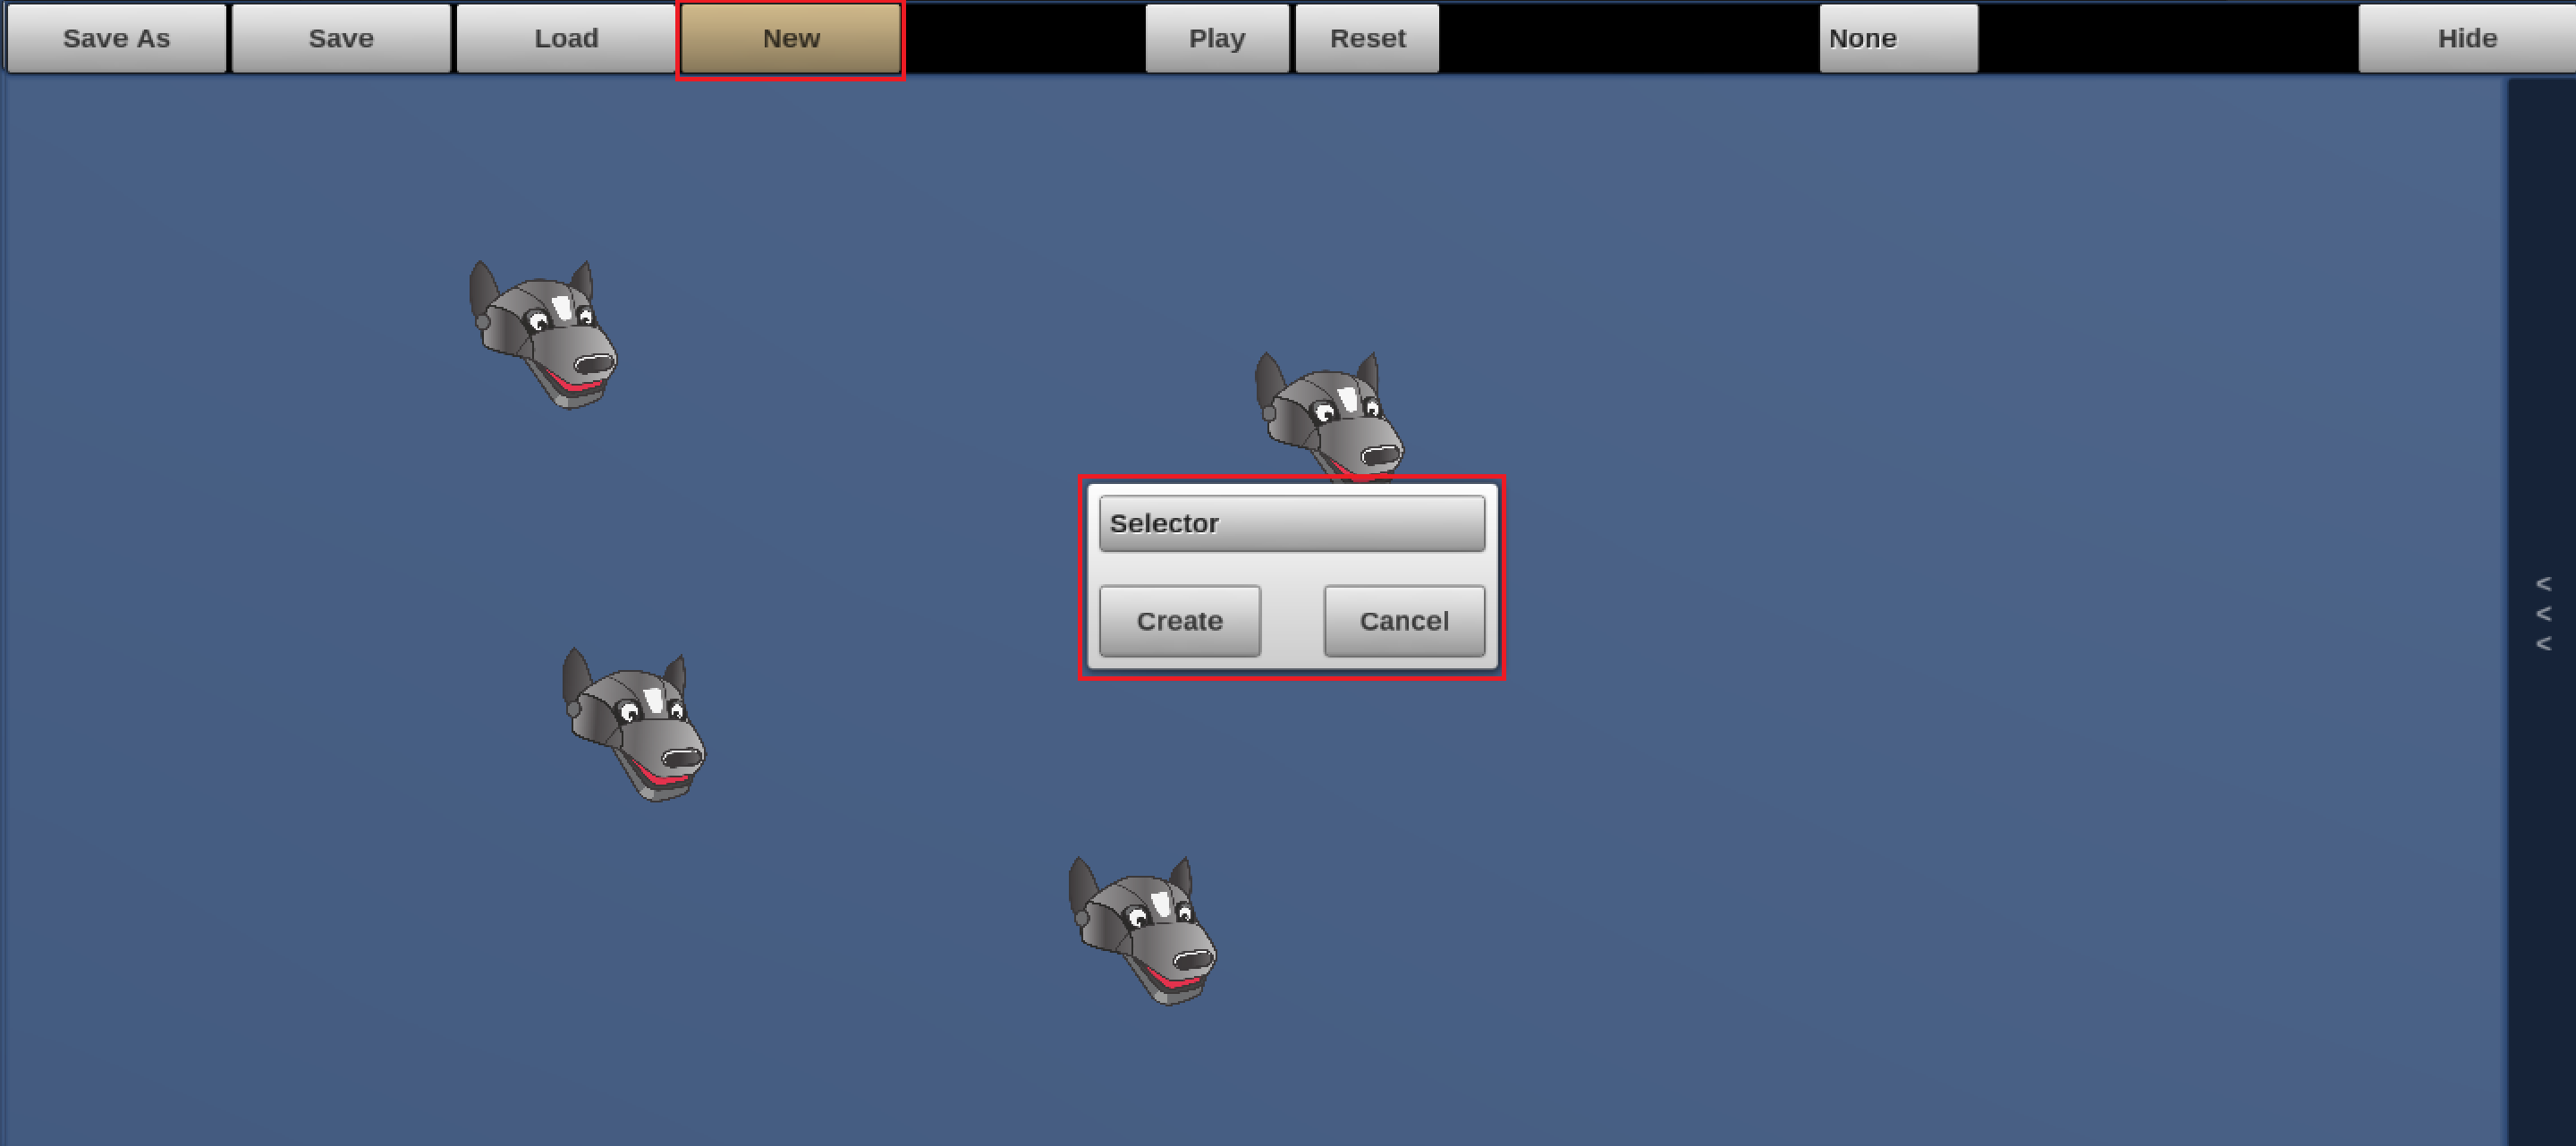
\includegraphics[width=1\textwidth]{images/KIAnleitung3_1}
	%\caption{Beziehung der BehaviourNode Klasse}
	\label{a2}
\end{figure}



\section{Bearbeiten}
Am rechten Rand verbirgt sich das Bearbeitungs-Men�. Mit einem Klick auf den schmalen Balken klappt sich dieses auf.

\begin{figure}[h!] %[hbtp]
	\centering
		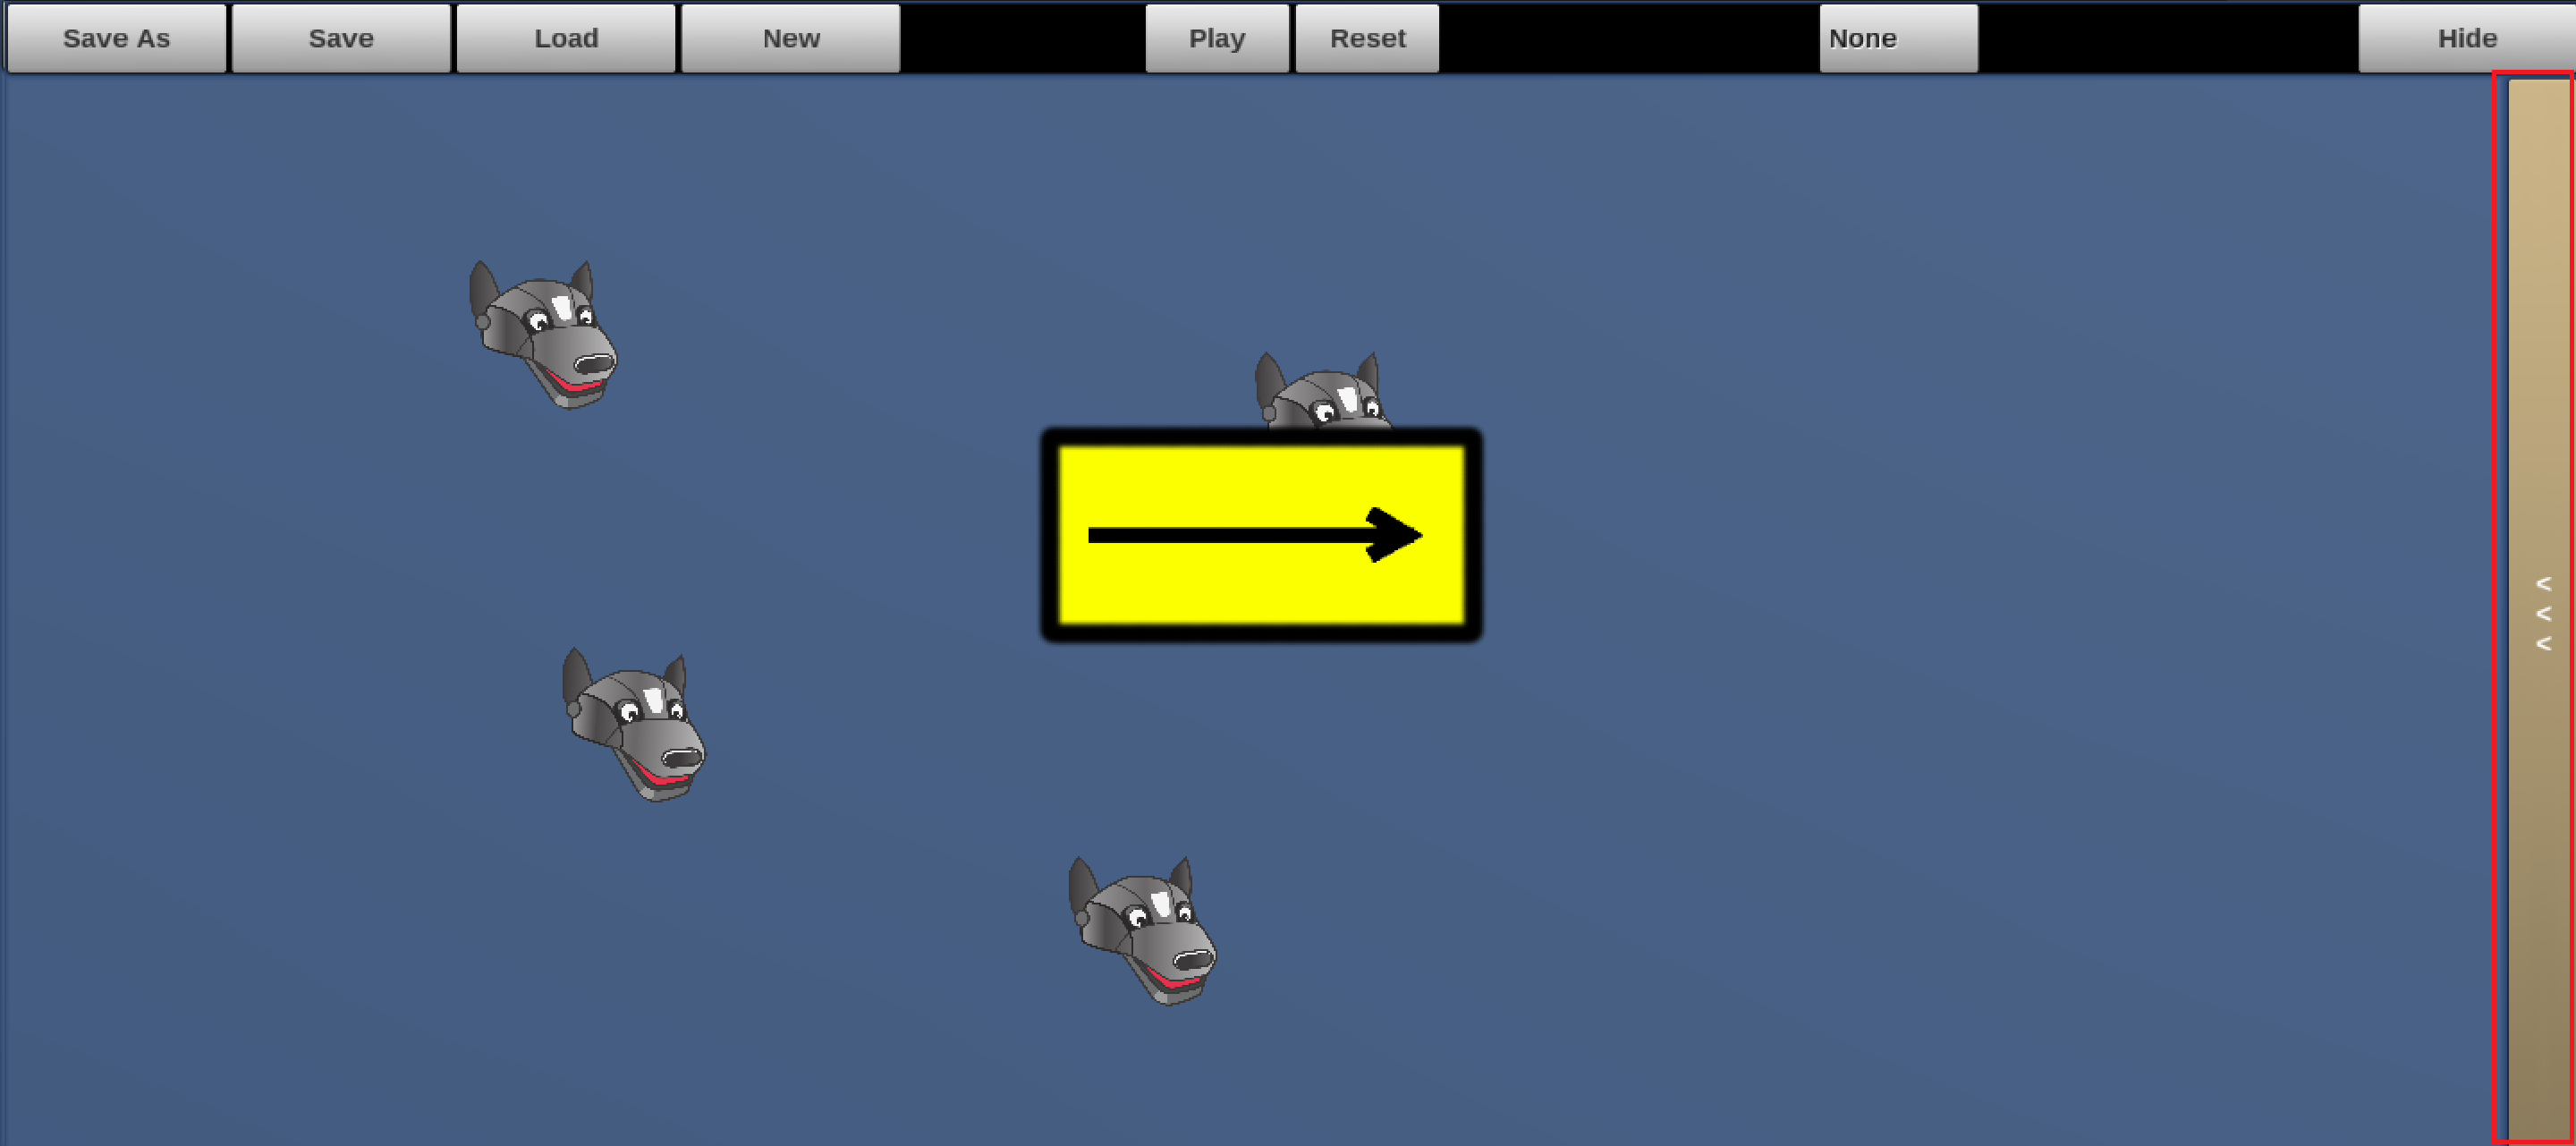
\includegraphics[width=1\textwidth]{images/KIAnleitung4_1}
	%\caption{Beziehung der BehaviourNode Klasse}
	\label{a3}
\end{figure}

\section{Knoten Ausw�hlen}
Mit einem Klick auf den zu bearbeitenden Knoten direkt im Baum dieser direkt ausgew�hlt und ist dadurch bearbeitbar.

\begin{figure}[h!] %[hbtp]
	\centering
		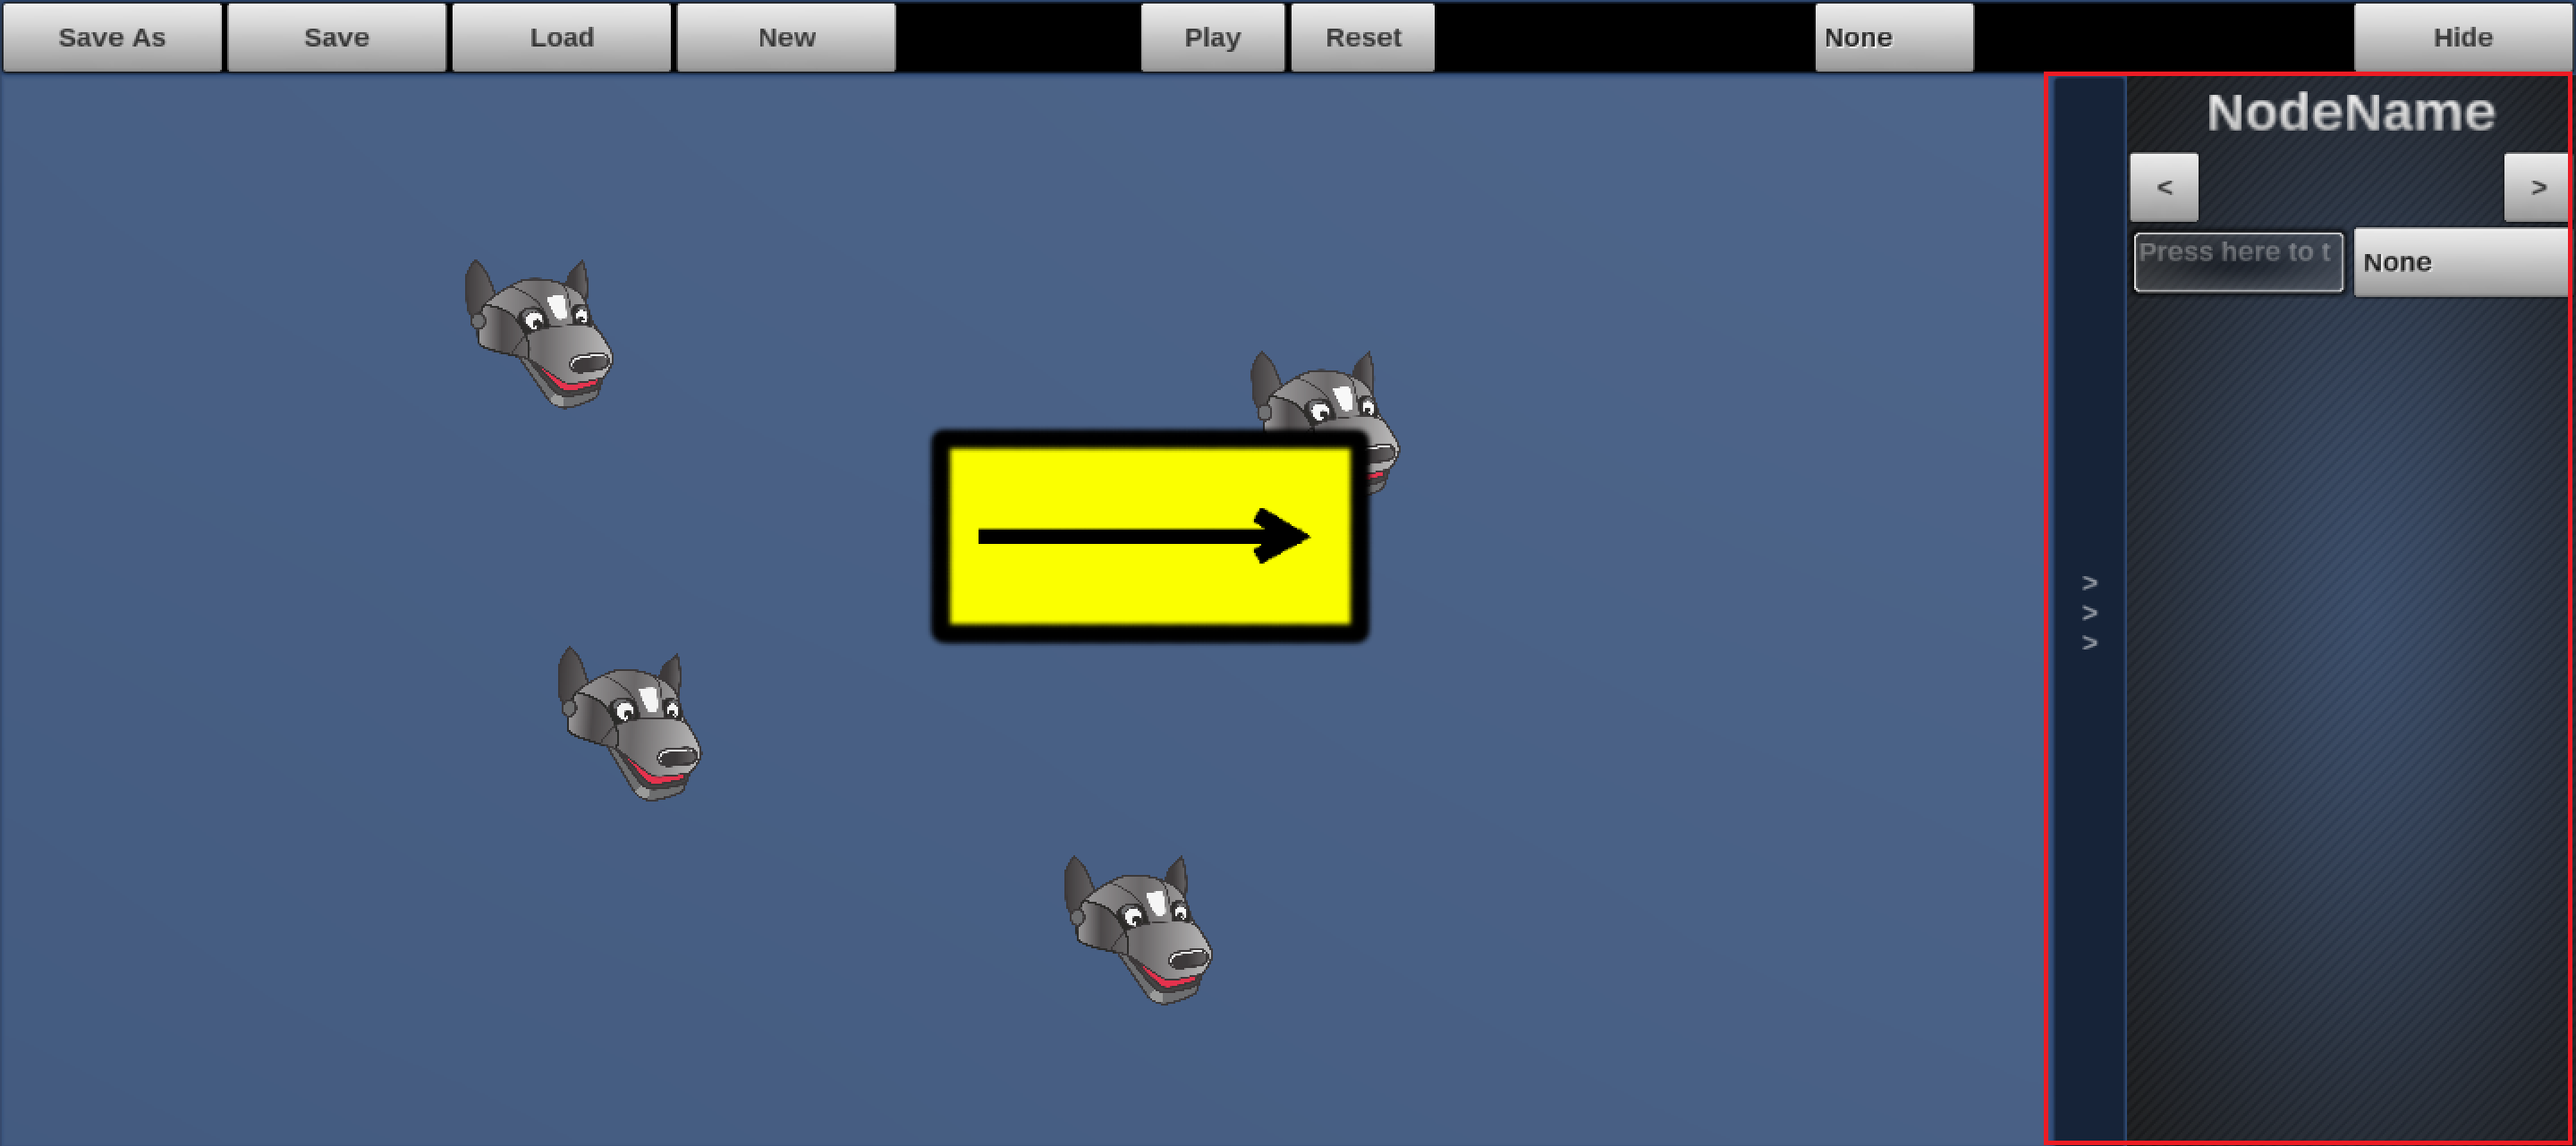
\includegraphics[width=1\textwidth]{images/KIAnleitung5_1}
	%\caption{Beziehung der BehaviourNode Klasse}
	\label{a4}
\end{figure}

\section{Unterknoten anlegen}
Wenn ein Vaterknoten ausgew�hlt ist, l�sst sich �ber die Liste im Bearbeitungsfenster ein neuer Task als Unterknoten hinzuf�gen. Um die Liste einzuschr�nken dient die Suchfunktion, welche auf Gro�- und Kleinschreibung achtet.

\begin{figure}[h!] %[hbtp]
	\centering
		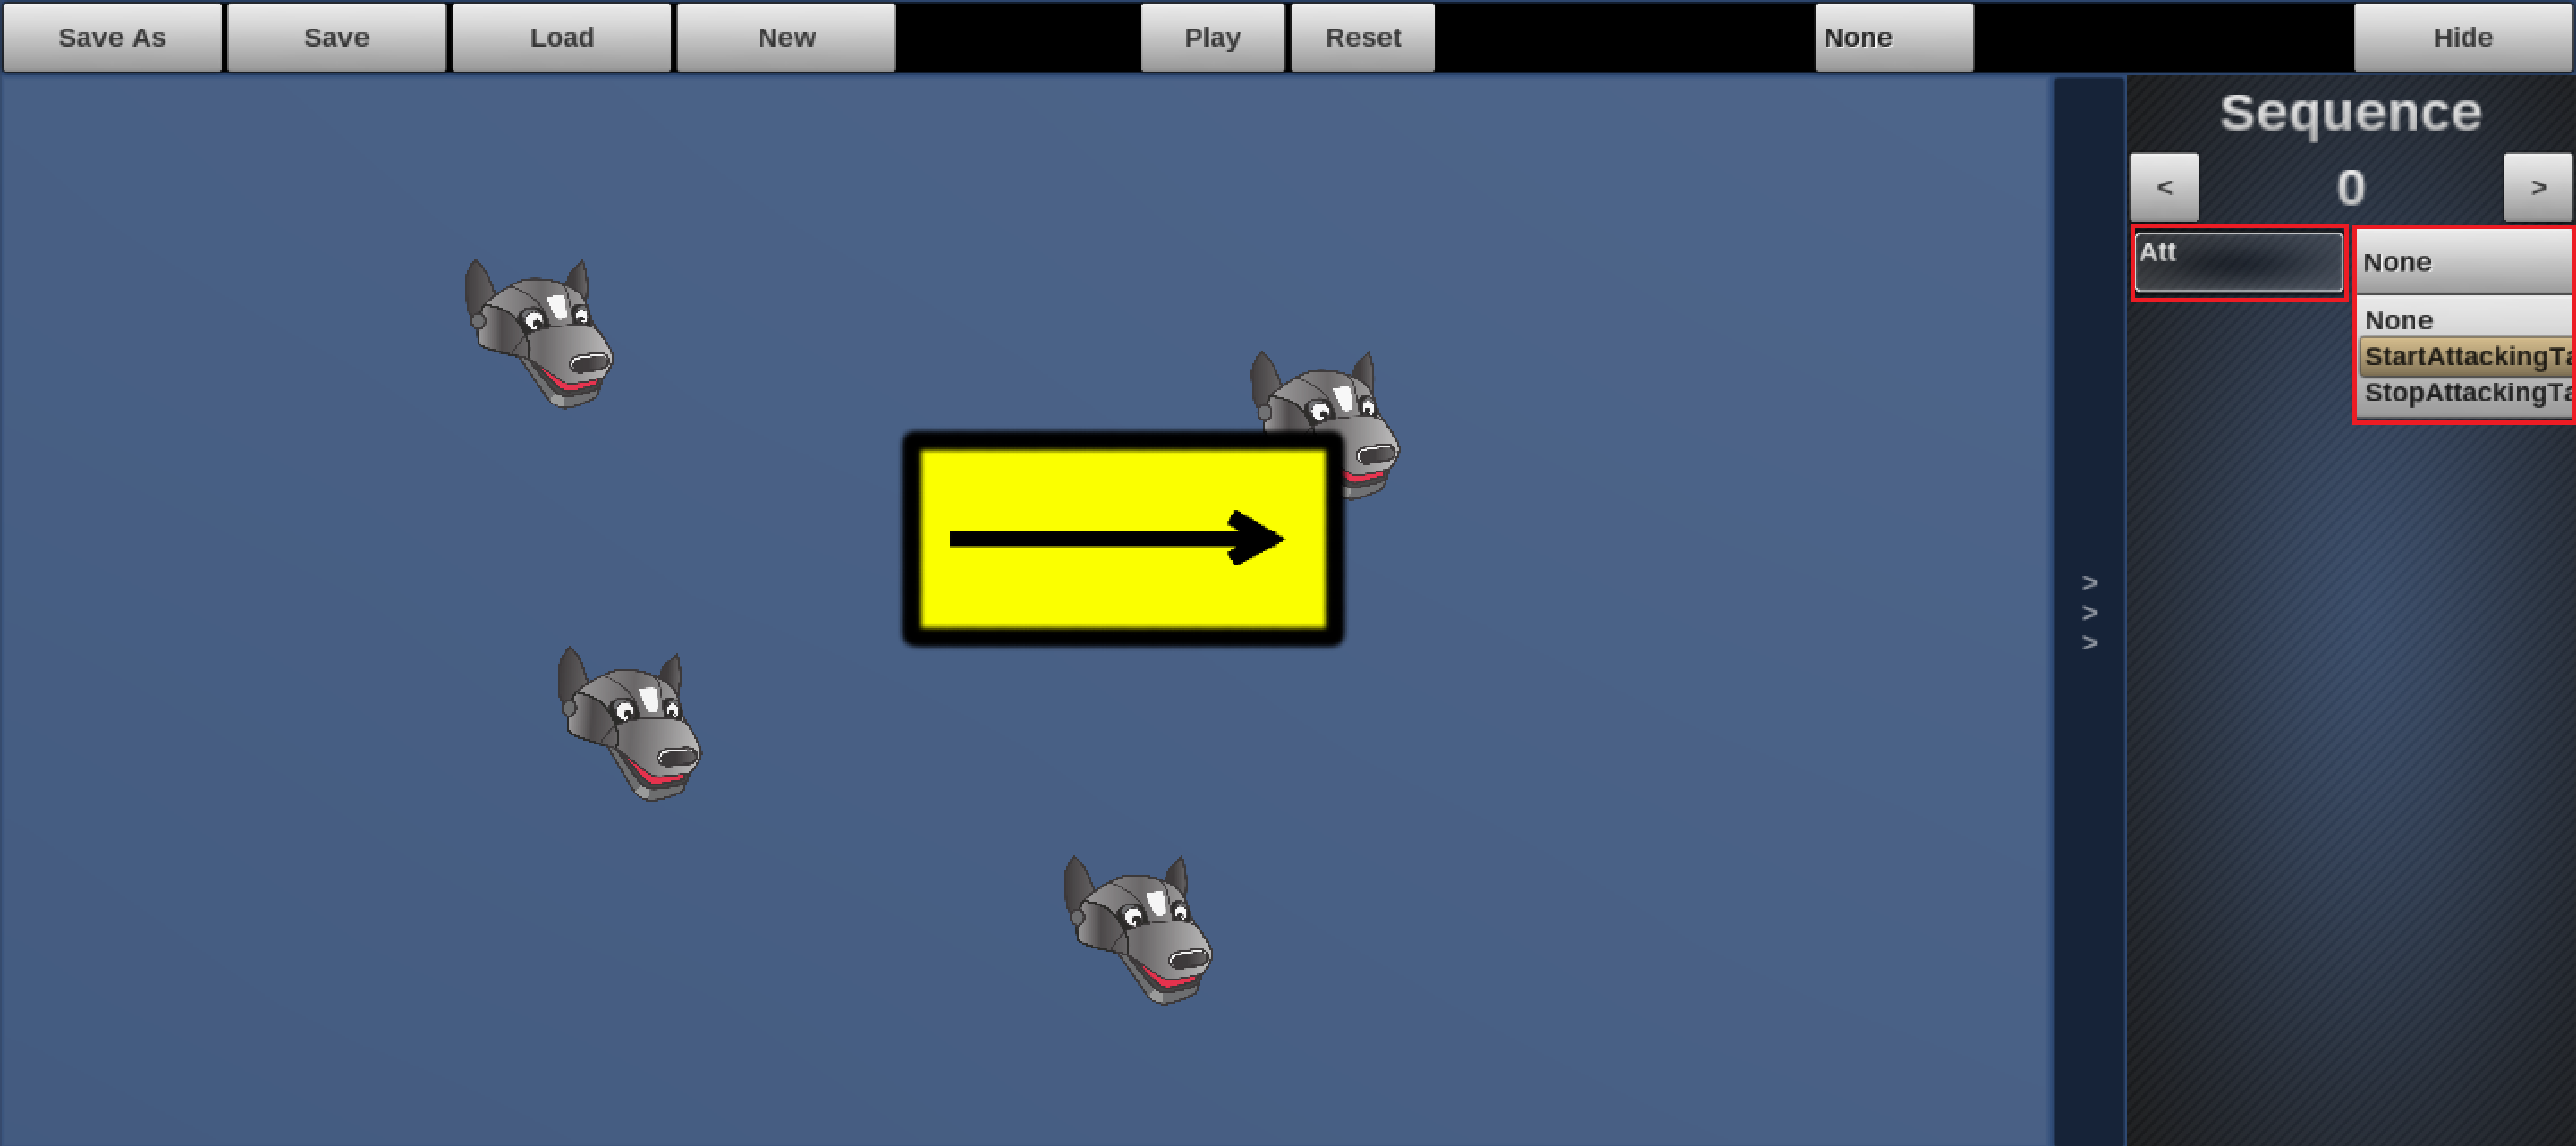
\includegraphics[width=1\textwidth]{images/KIAnleitung55_1}
	%\caption{Beziehung der BehaviourNode Klasse}
	\label{a5}
\end{figure}

\begin{figure}[h!] %[hbtp]
	\centering
		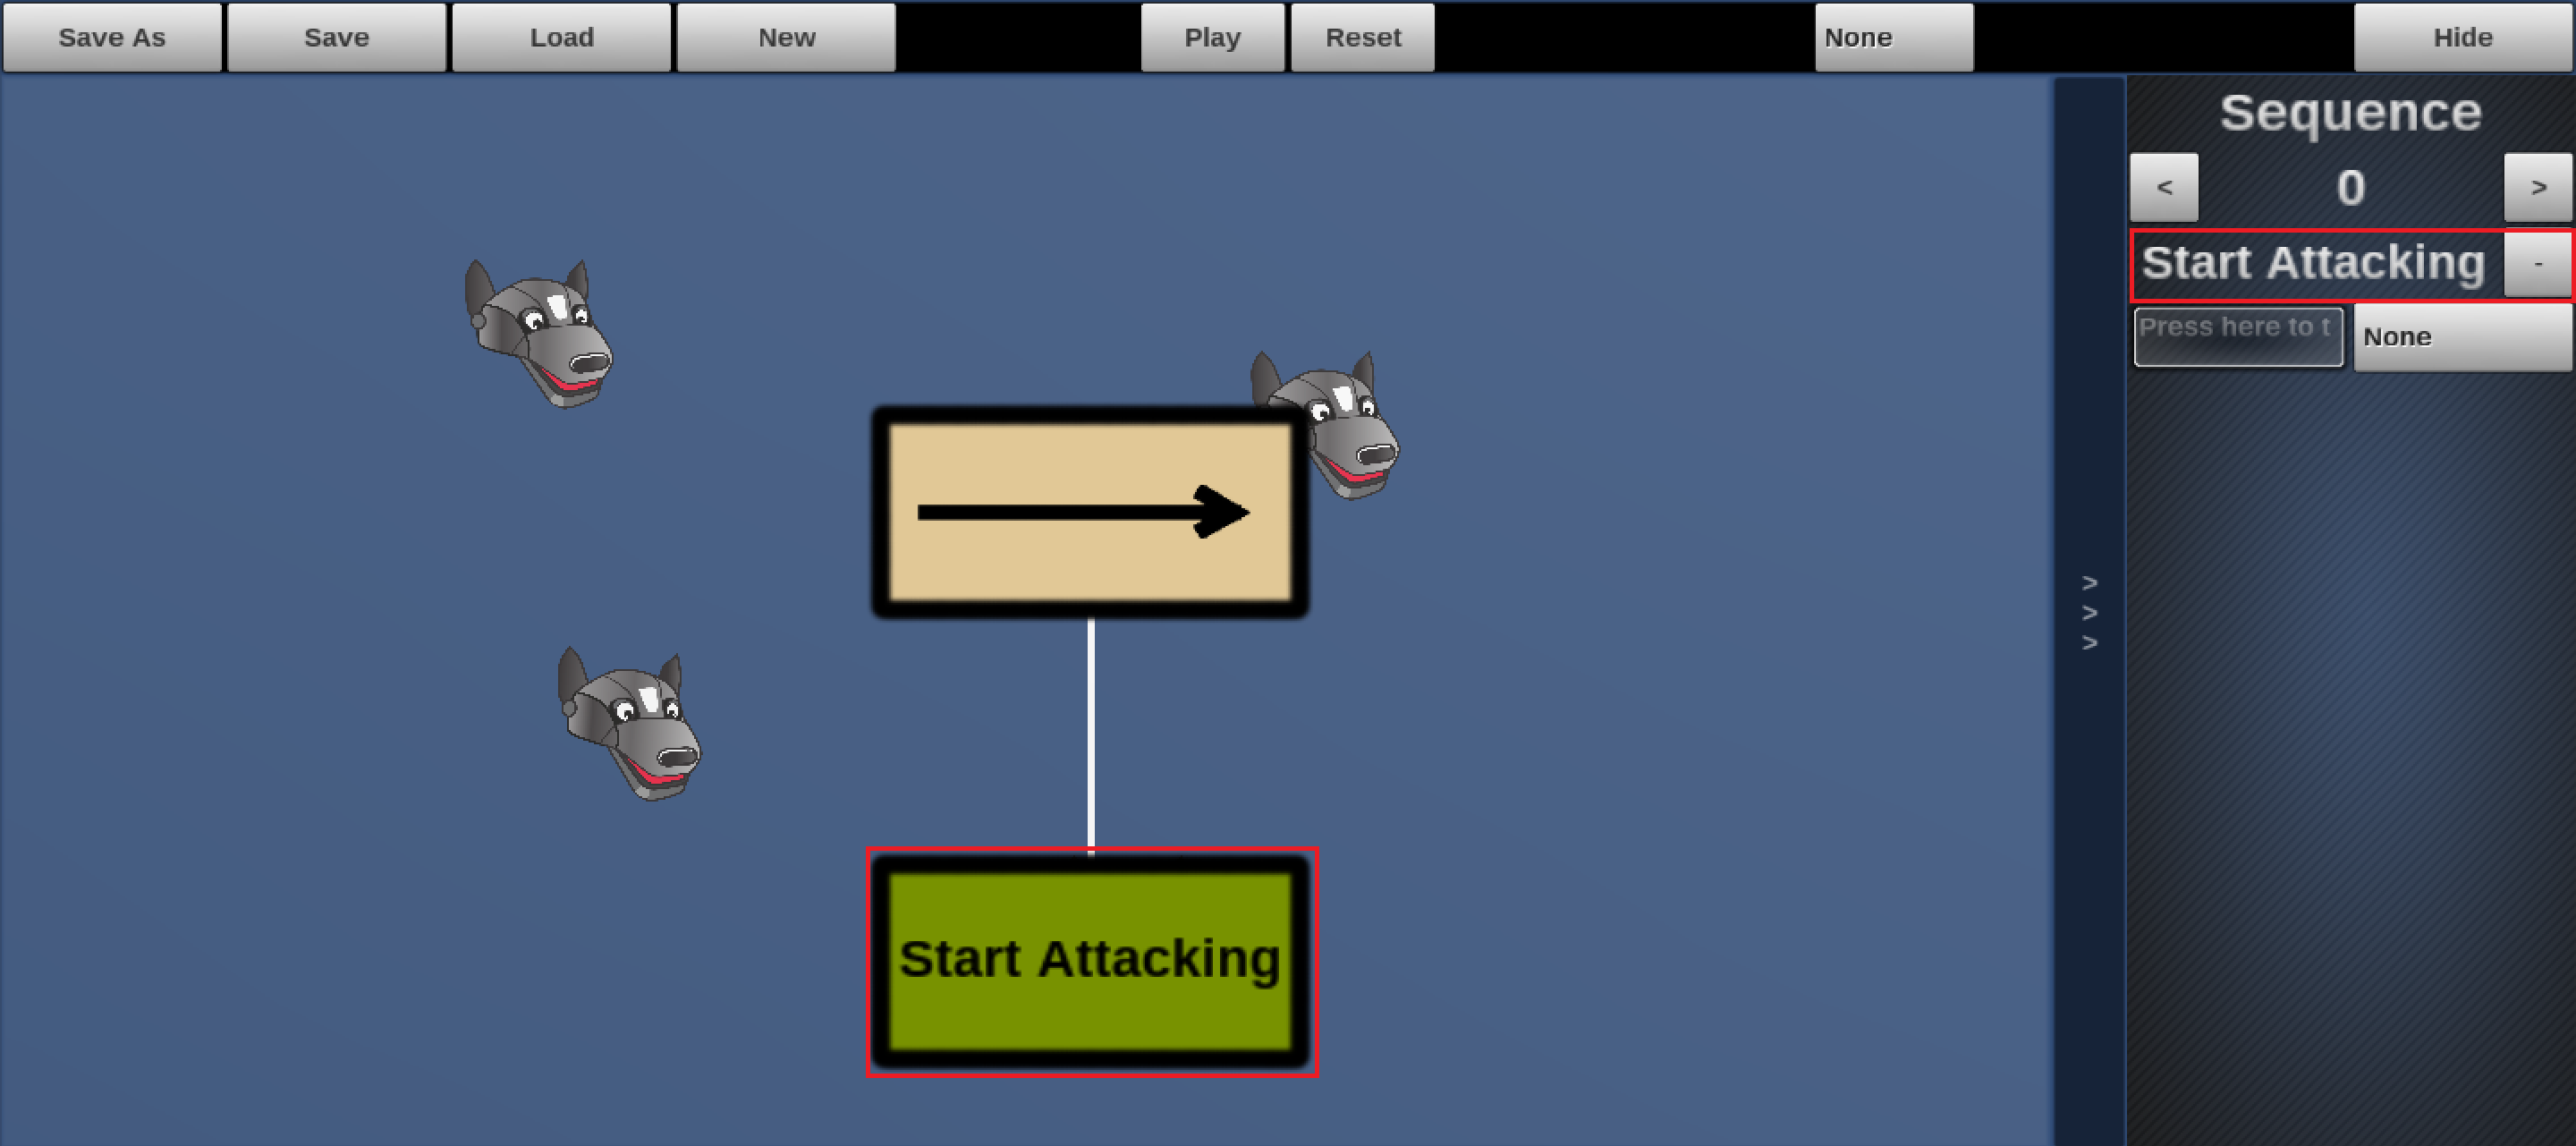
\includegraphics[width=1\textwidth]{images/KIAnleitung555_1}
	%\caption{Beziehung der BehaviourNode Klasse}
	\label{a6}
\end{figure}



\section{Knoten verschieben}
Direkt unter dem Namen des Knotens befindet sich deine Index-Position in der Reihe der Unterknoten. Mit einem Klick auf den Links- oder Rechts-Buttons wird der Knoten in der Reihe dementsprechend verschoben.
\begin{figure}[h!] %[hbtp]
	\centering
		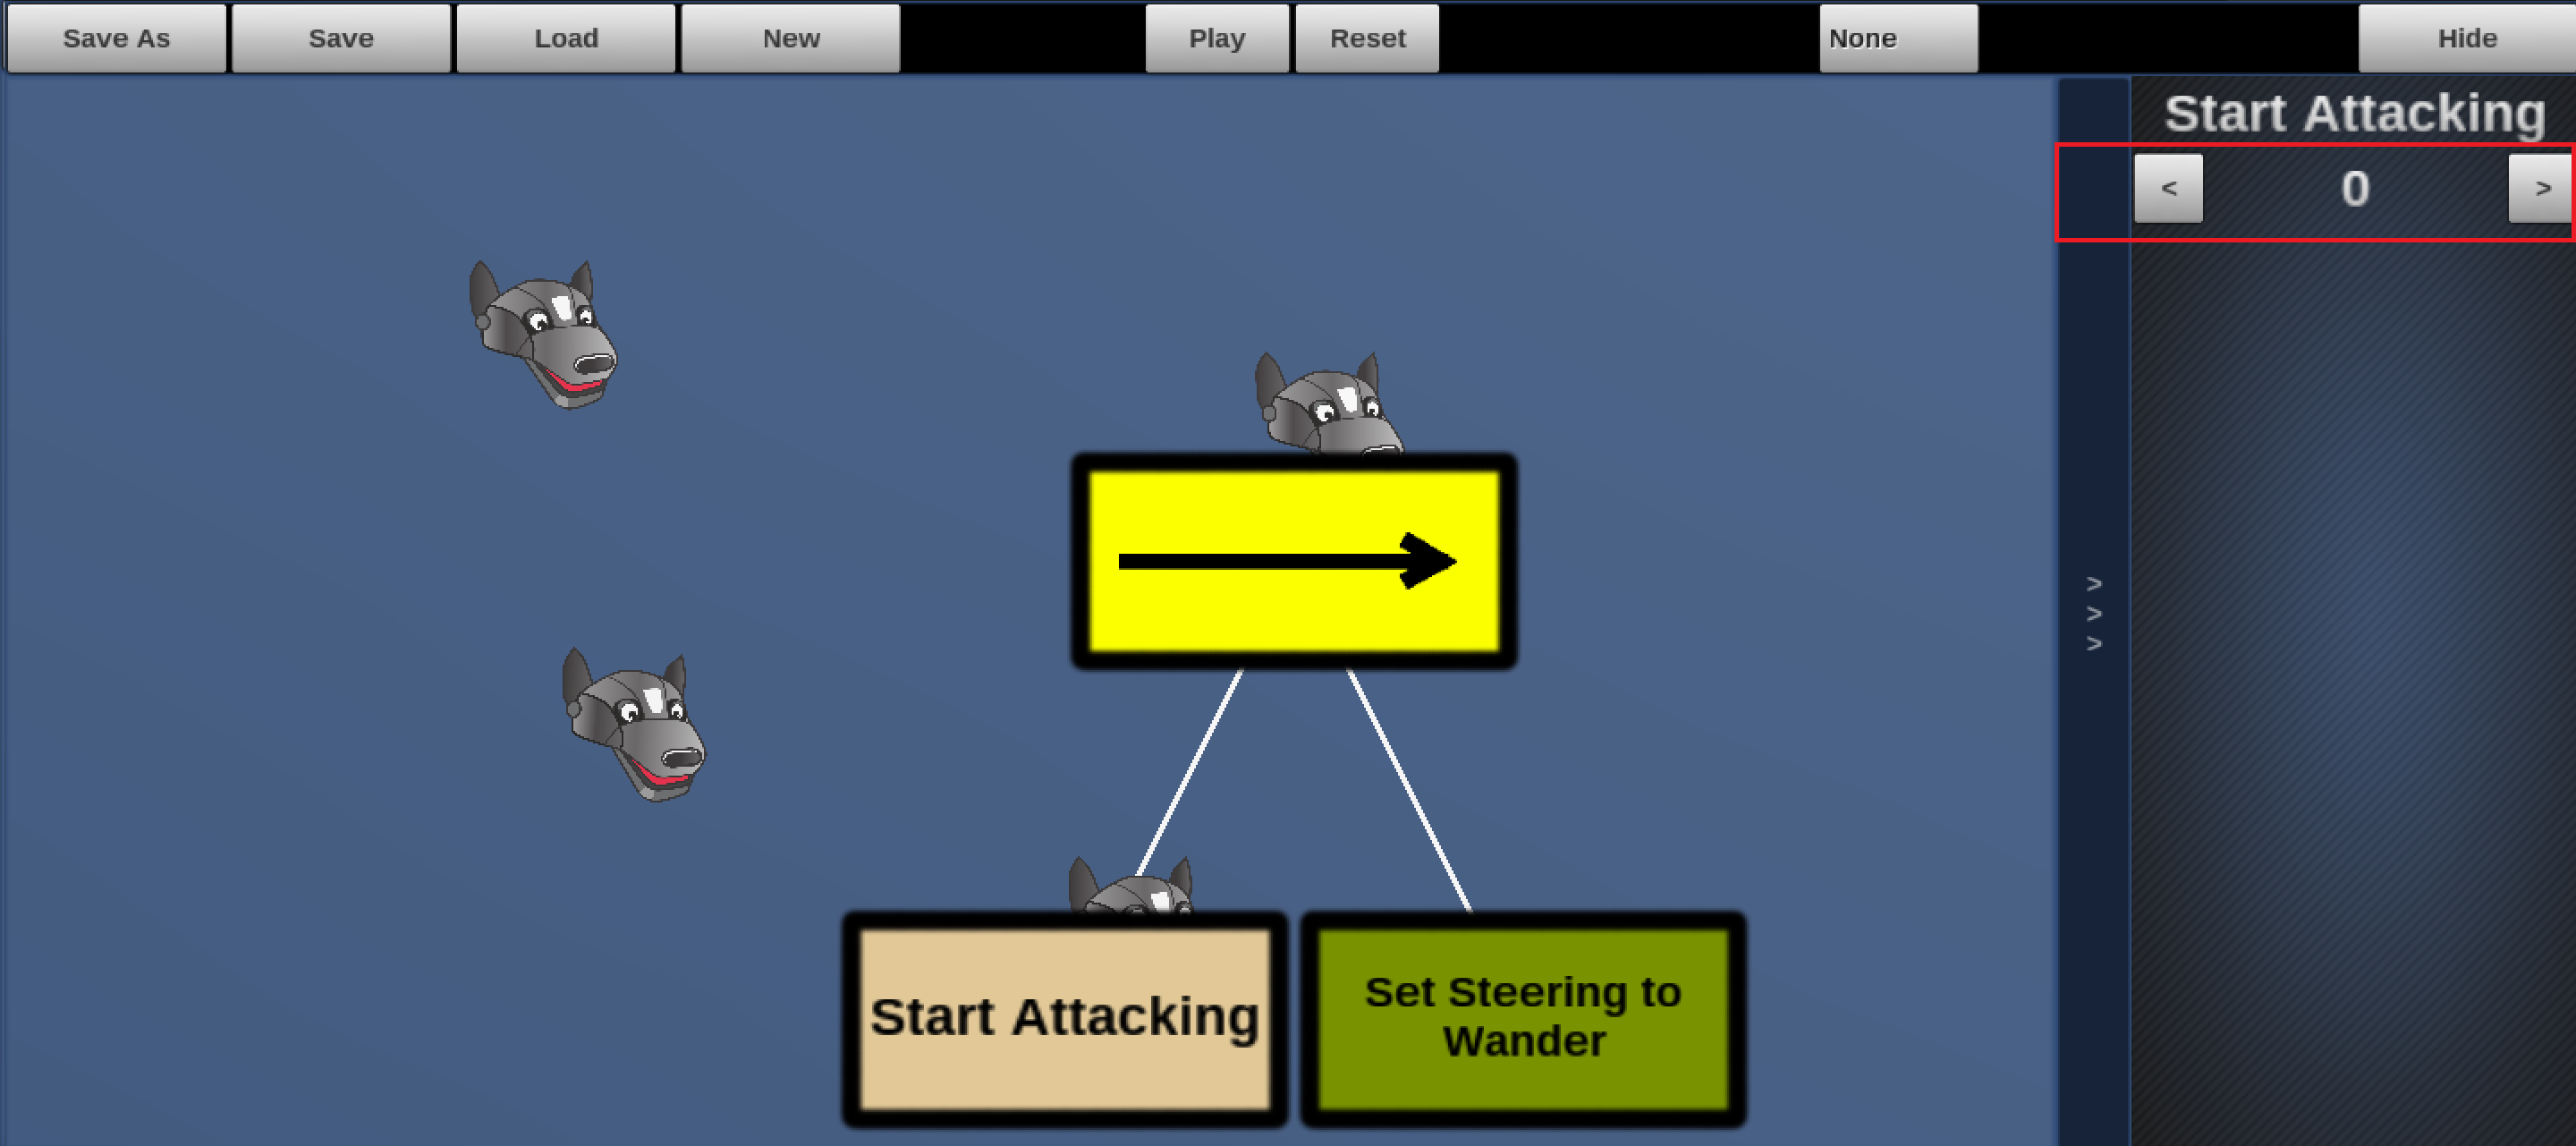
\includegraphics[width=1\textwidth]{images/KIAnleitung6_1}
	%\caption{Beziehung der BehaviourNode Klasse}
	\label{a7}
\end{figure}

\begin{figure}[h!] %[hbtp]
	\centering
		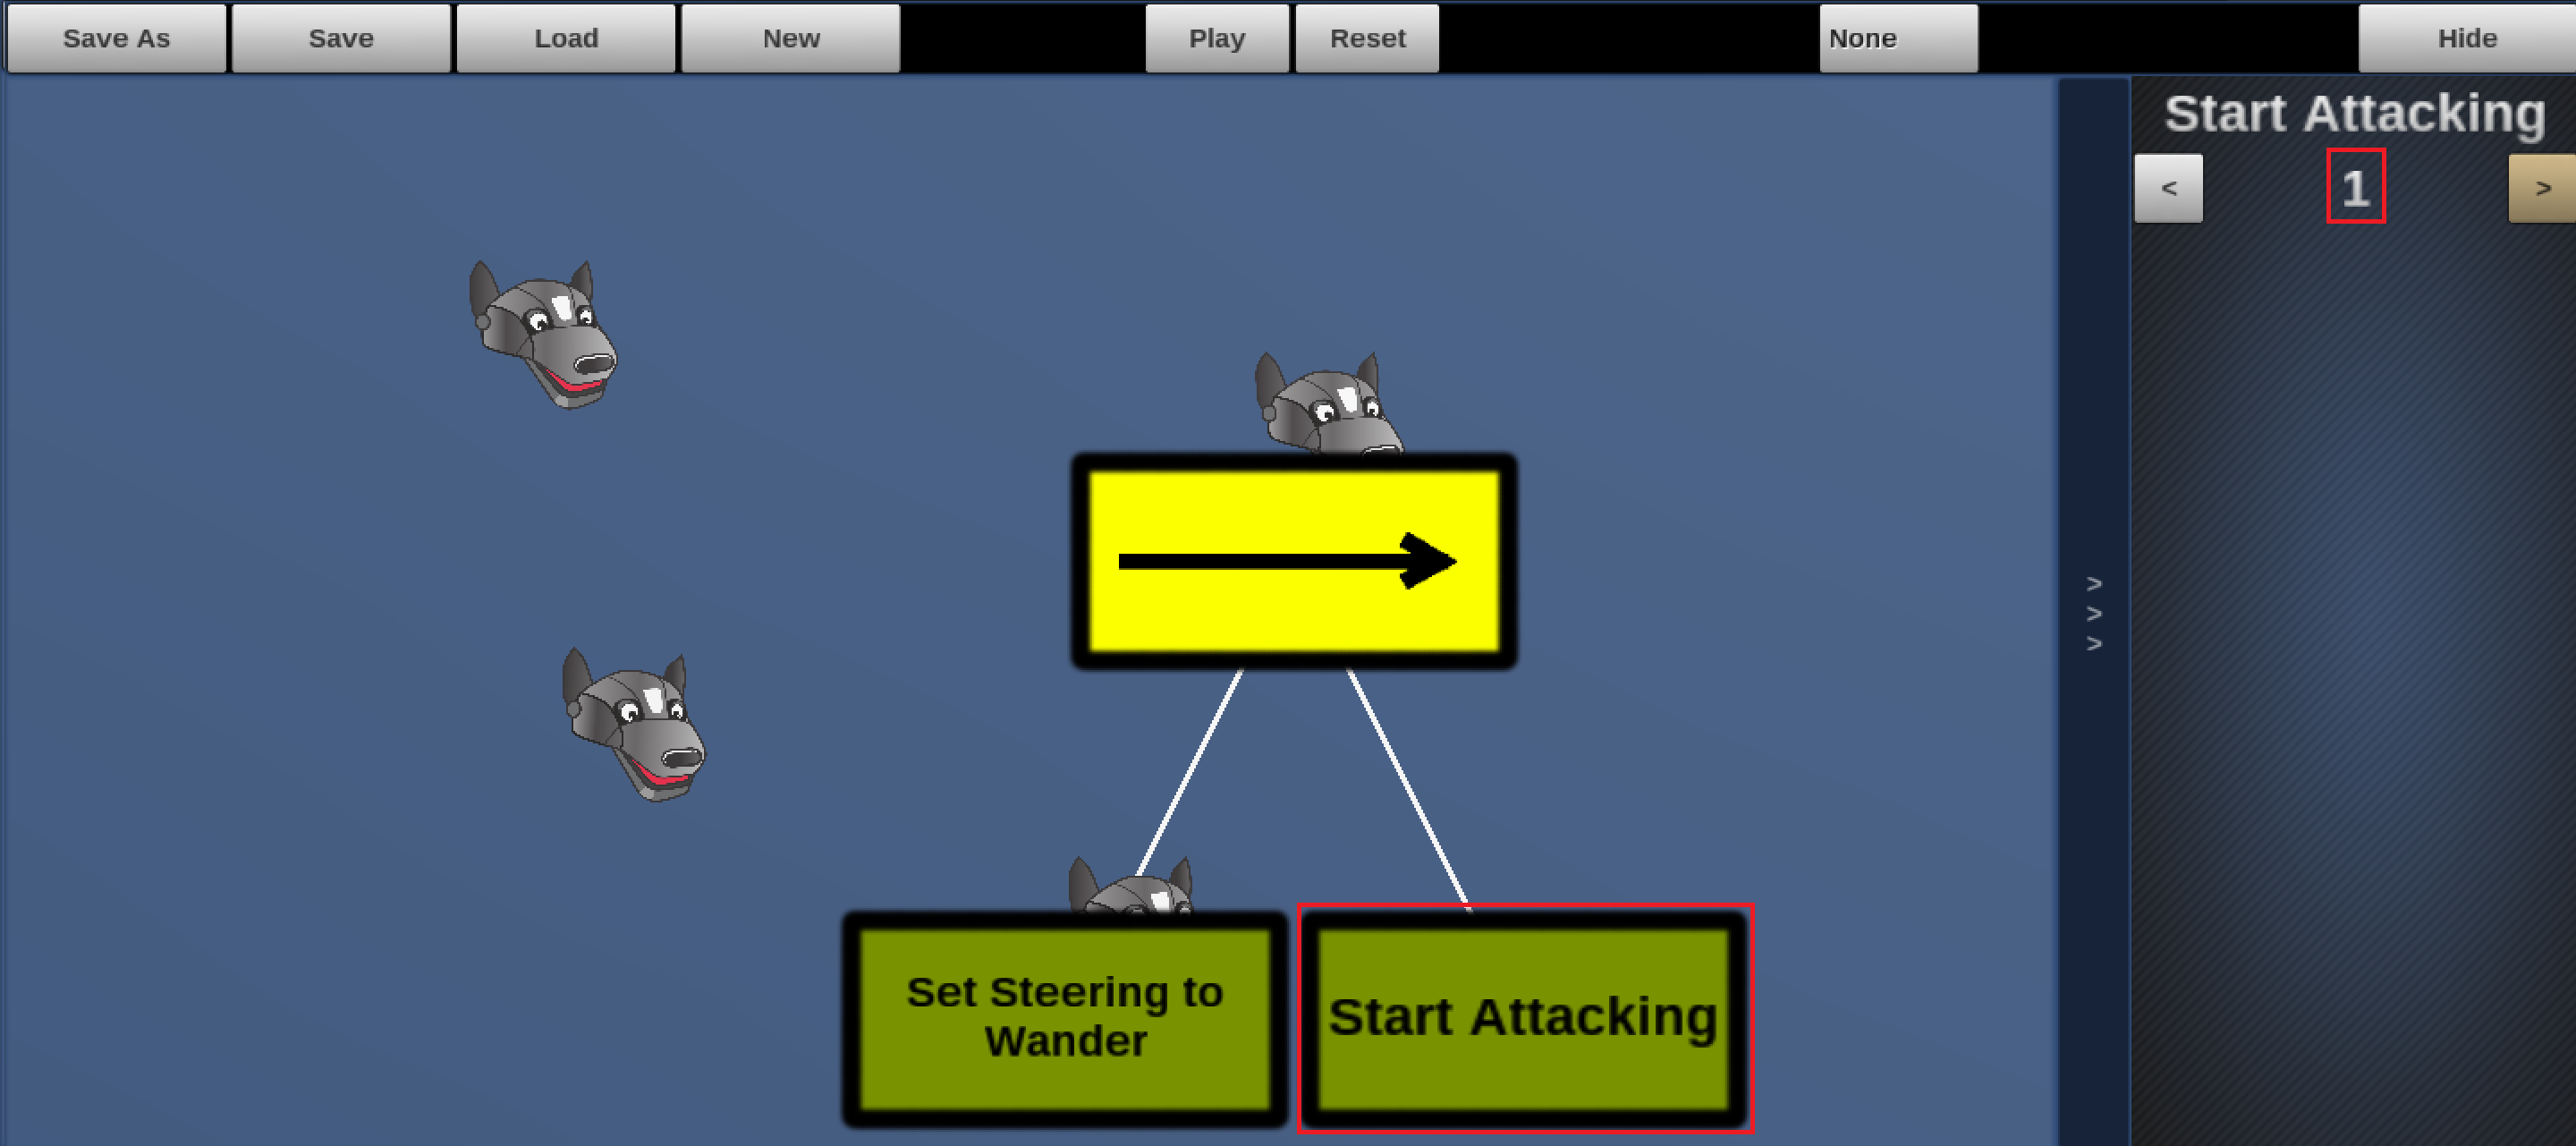
\includegraphics[width=1\textwidth]{images/KIAnleitung7_1}
	%\caption{Beziehung der BehaviourNode Klasse}
	\label{a8}
\end{figure}


\section{Knoten l�schen}
Um einen Knoten zu l�schen wird der Vaterknoten dessen ausgew�hlt. Dort stehen die Kind-Knoten aufgelistet. Rechts neben den Namen dieser befindet sich der L�schen-Button. Durch das anklicken wird der Knoten aus der Liste der Kindknoten entfernt.
\begin{figure}[h!] %[hbtp]
	\centering
		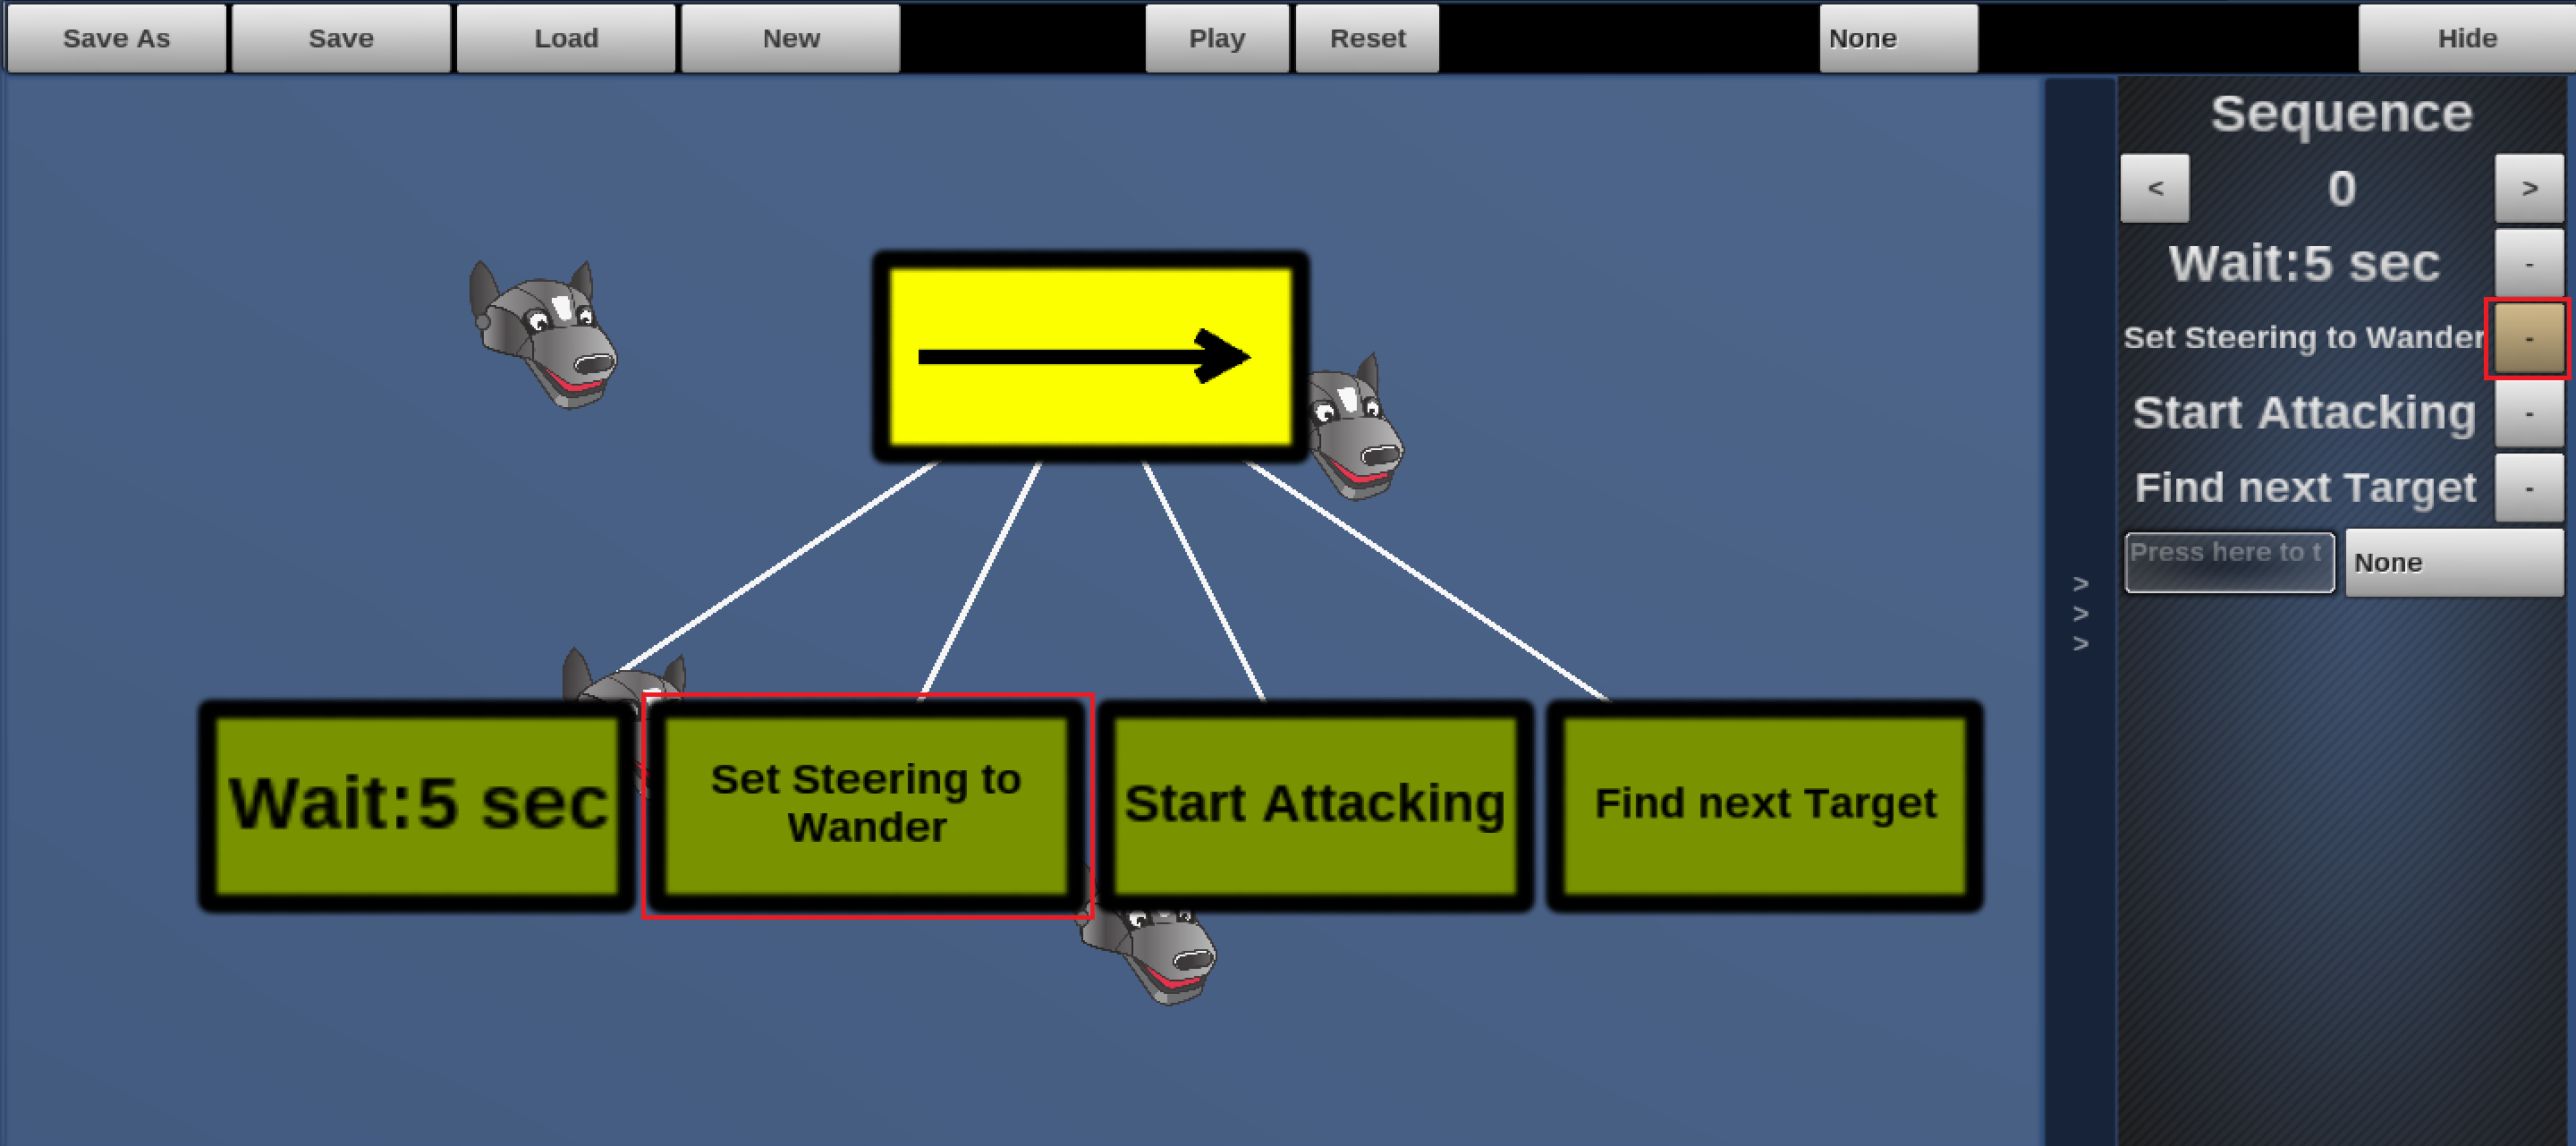
\includegraphics[width=1\textwidth]{images/KIAnleitung17_1}
	%\caption{Beziehung der BehaviourNode Klasse}
	\label{a9}
\end{figure}

\begin{figure}[h!] %[hbtp]
	\centering
		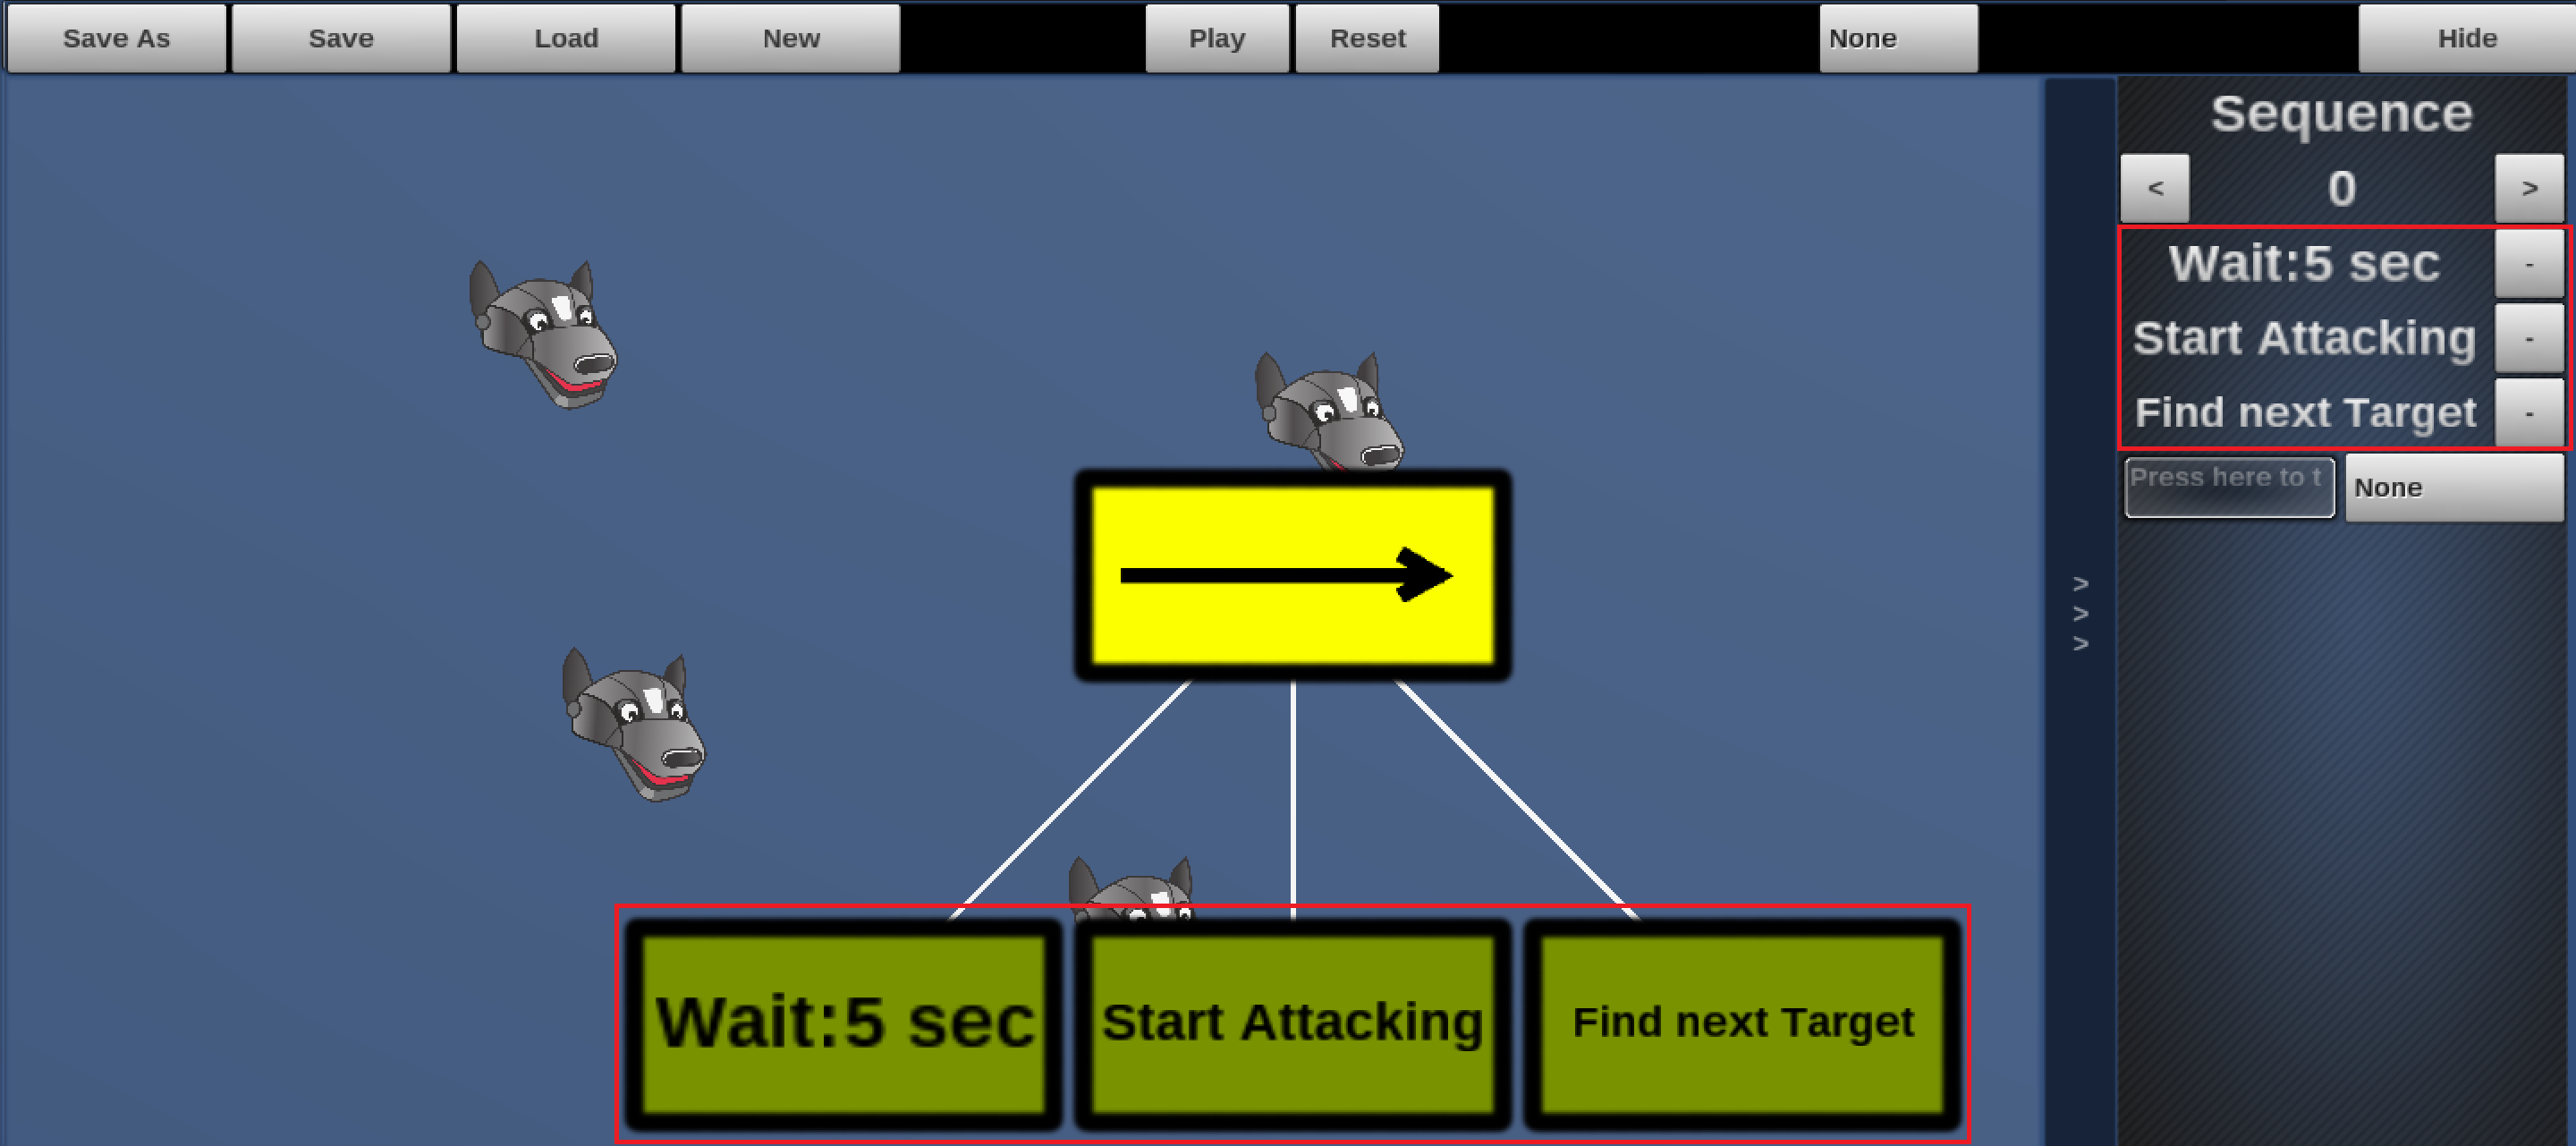
\includegraphics[width=1\textwidth]{images/KIAnleitung18_1}
	%\caption{Beziehung der BehaviourNode Klasse}
	\label{a10}
\end{figure}



\section{Speichern}
\subsection{Neuer Baum}
Beim Speichern eines neuen Baumes wird in der Leiste am oberen Bildschirmrand der "'Save As"'-Button ausgew�hlt. Dadurch �ffnet sich ein Fenster in welchem der Name f�r den Baum eingegeben wird. Durch "Save" wird der Baum abgespeichert.

\begin{figure}[h!] %[hbtp]
	\centering
		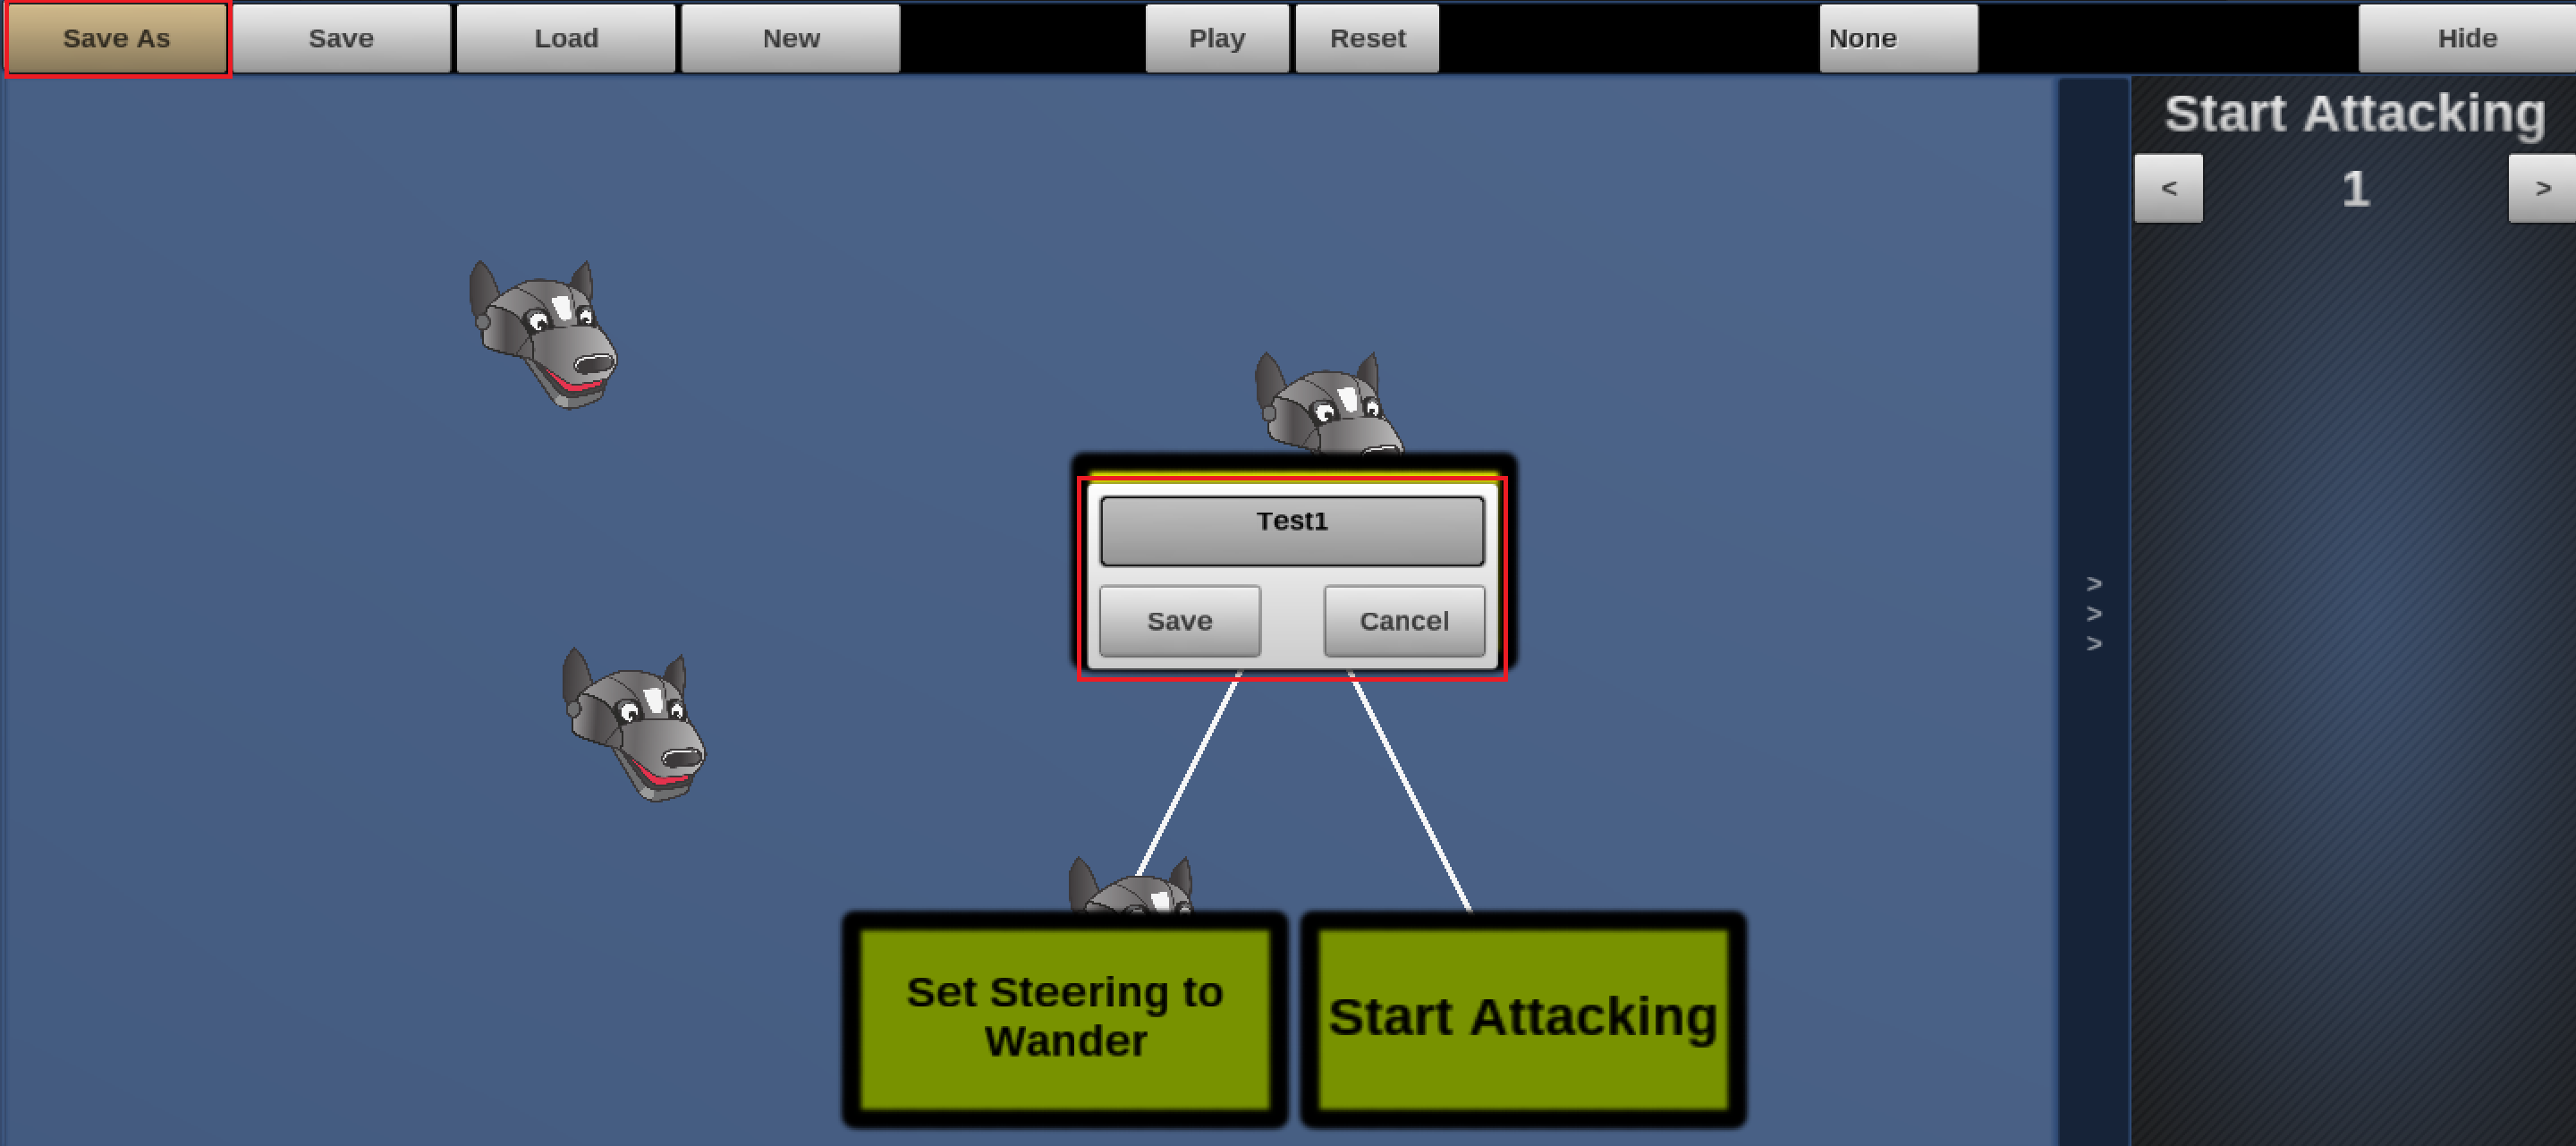
\includegraphics[width=1\textwidth]{images/KIAnleitung8_1}
	%\caption{Beziehung der BehaviourNode Klasse}
	\label{a11}
\end{figure}
\subsection{Bereits vorhandener Baum}
Wenn ein bereits gespeicherter Baum ver�ndert wurde, kann der Fortschritt durch den Save-Button gesichert werden.

\begin{figure}[h!] %[hbtp]
	\centering
		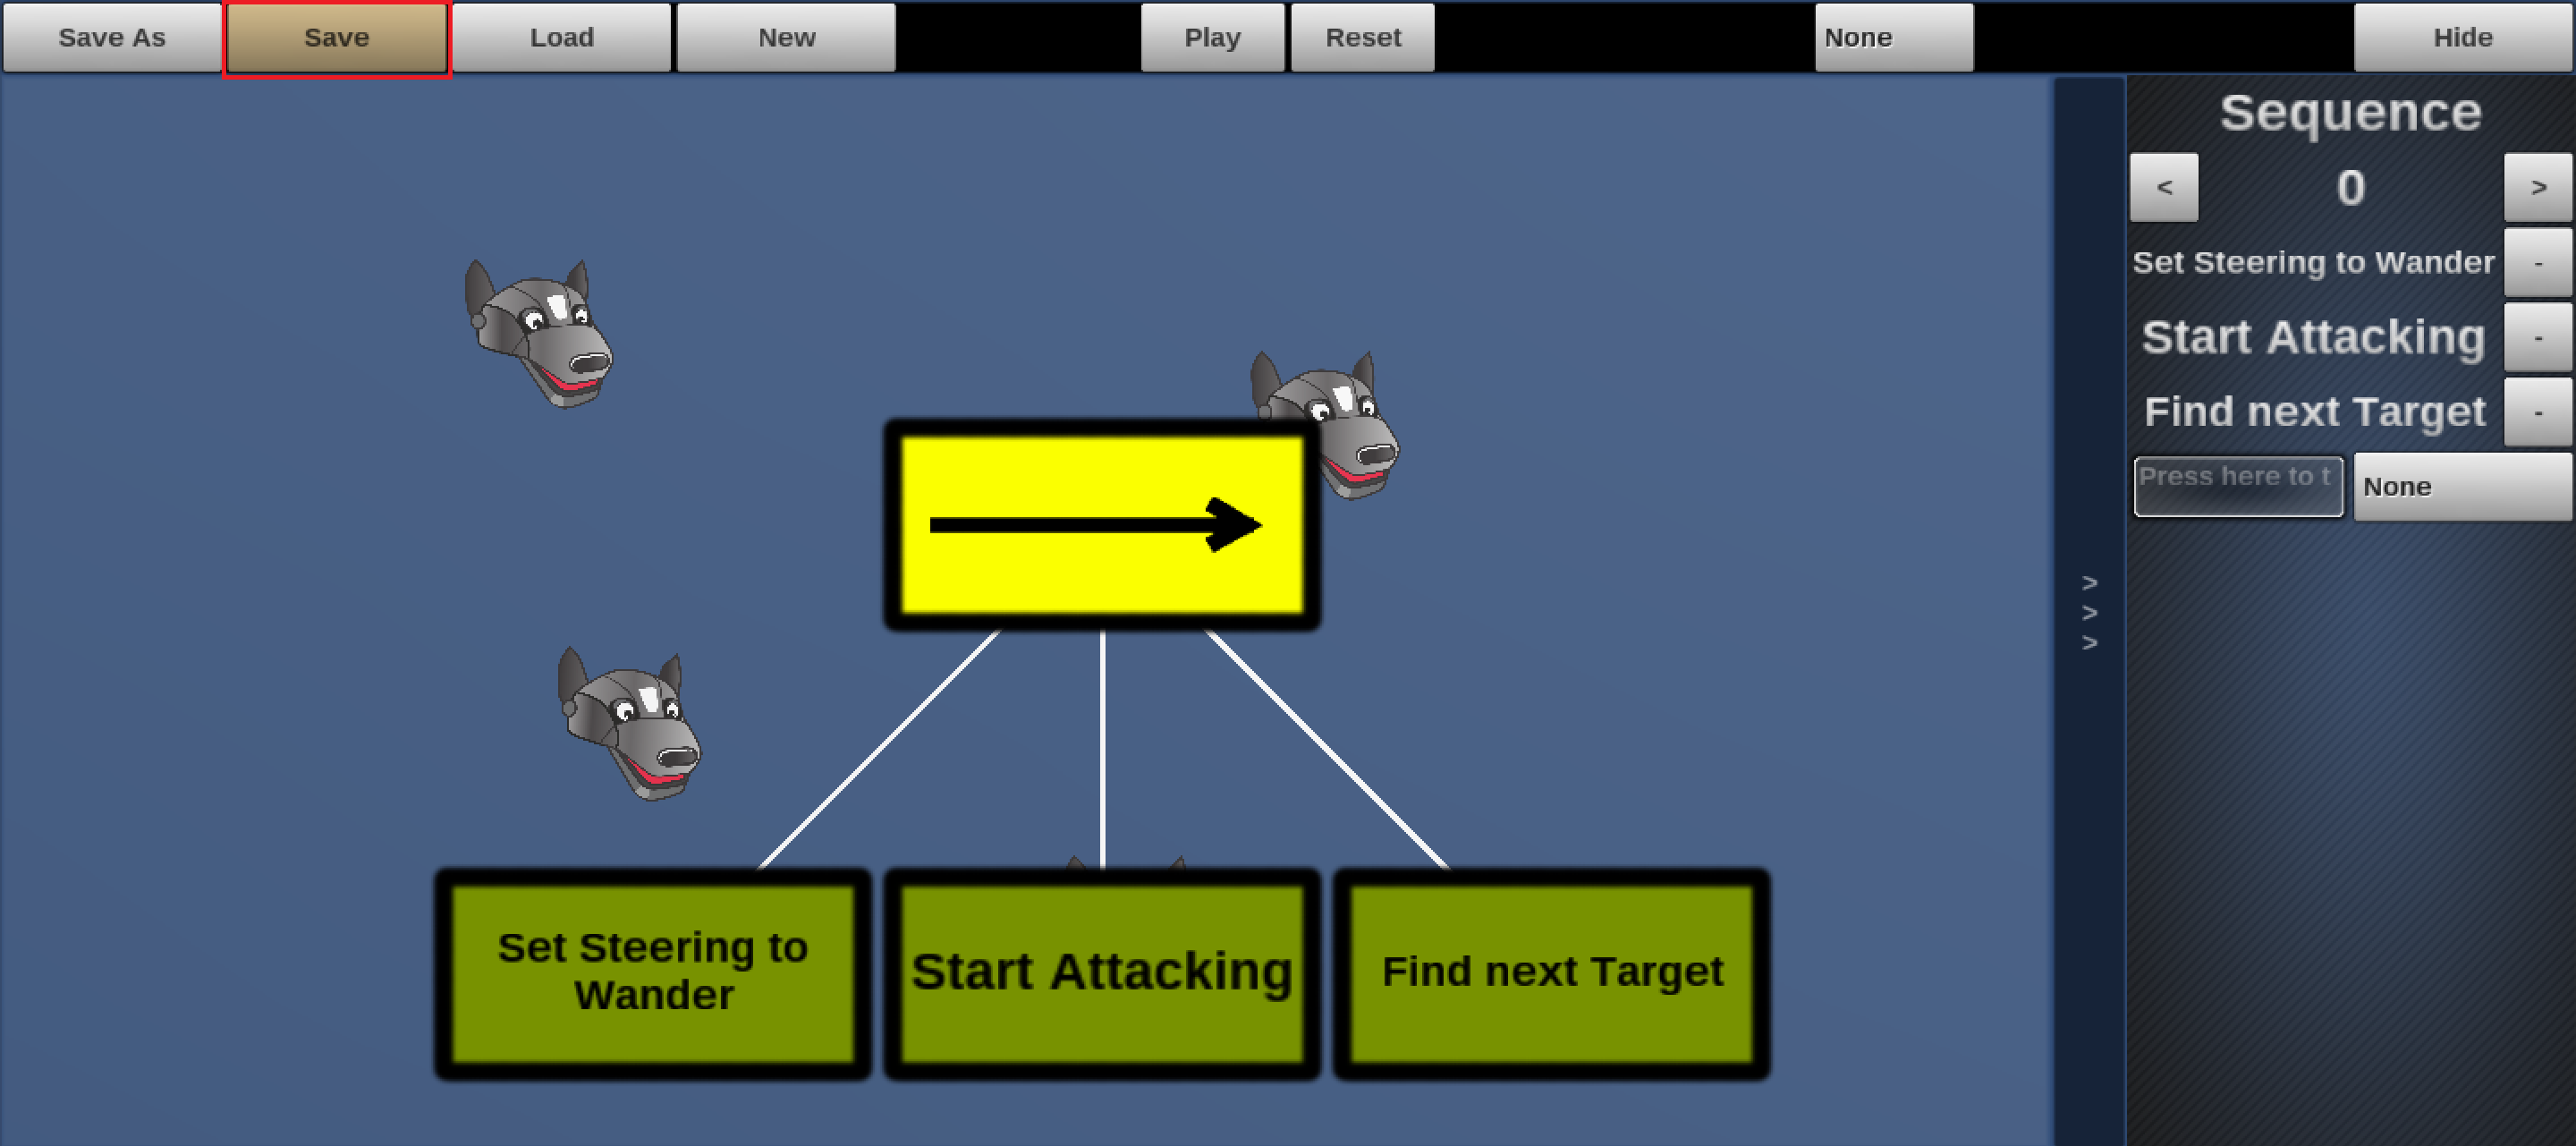
\includegraphics[width=1\textwidth]{images/KIAnleitung9_1}
	%\caption{Beziehung der BehaviourNode Klasse}
	\label{a12}
\end{figure}


\section{Laden}
�ber den Load-Button am oberen Bildschirmrand kann aus einer Liste der gespeicherten B�ume ausgew�hlt werden um diesen weiter zu editieren. 
\begin{figure}[h!] %[hbtp]
	\centering
		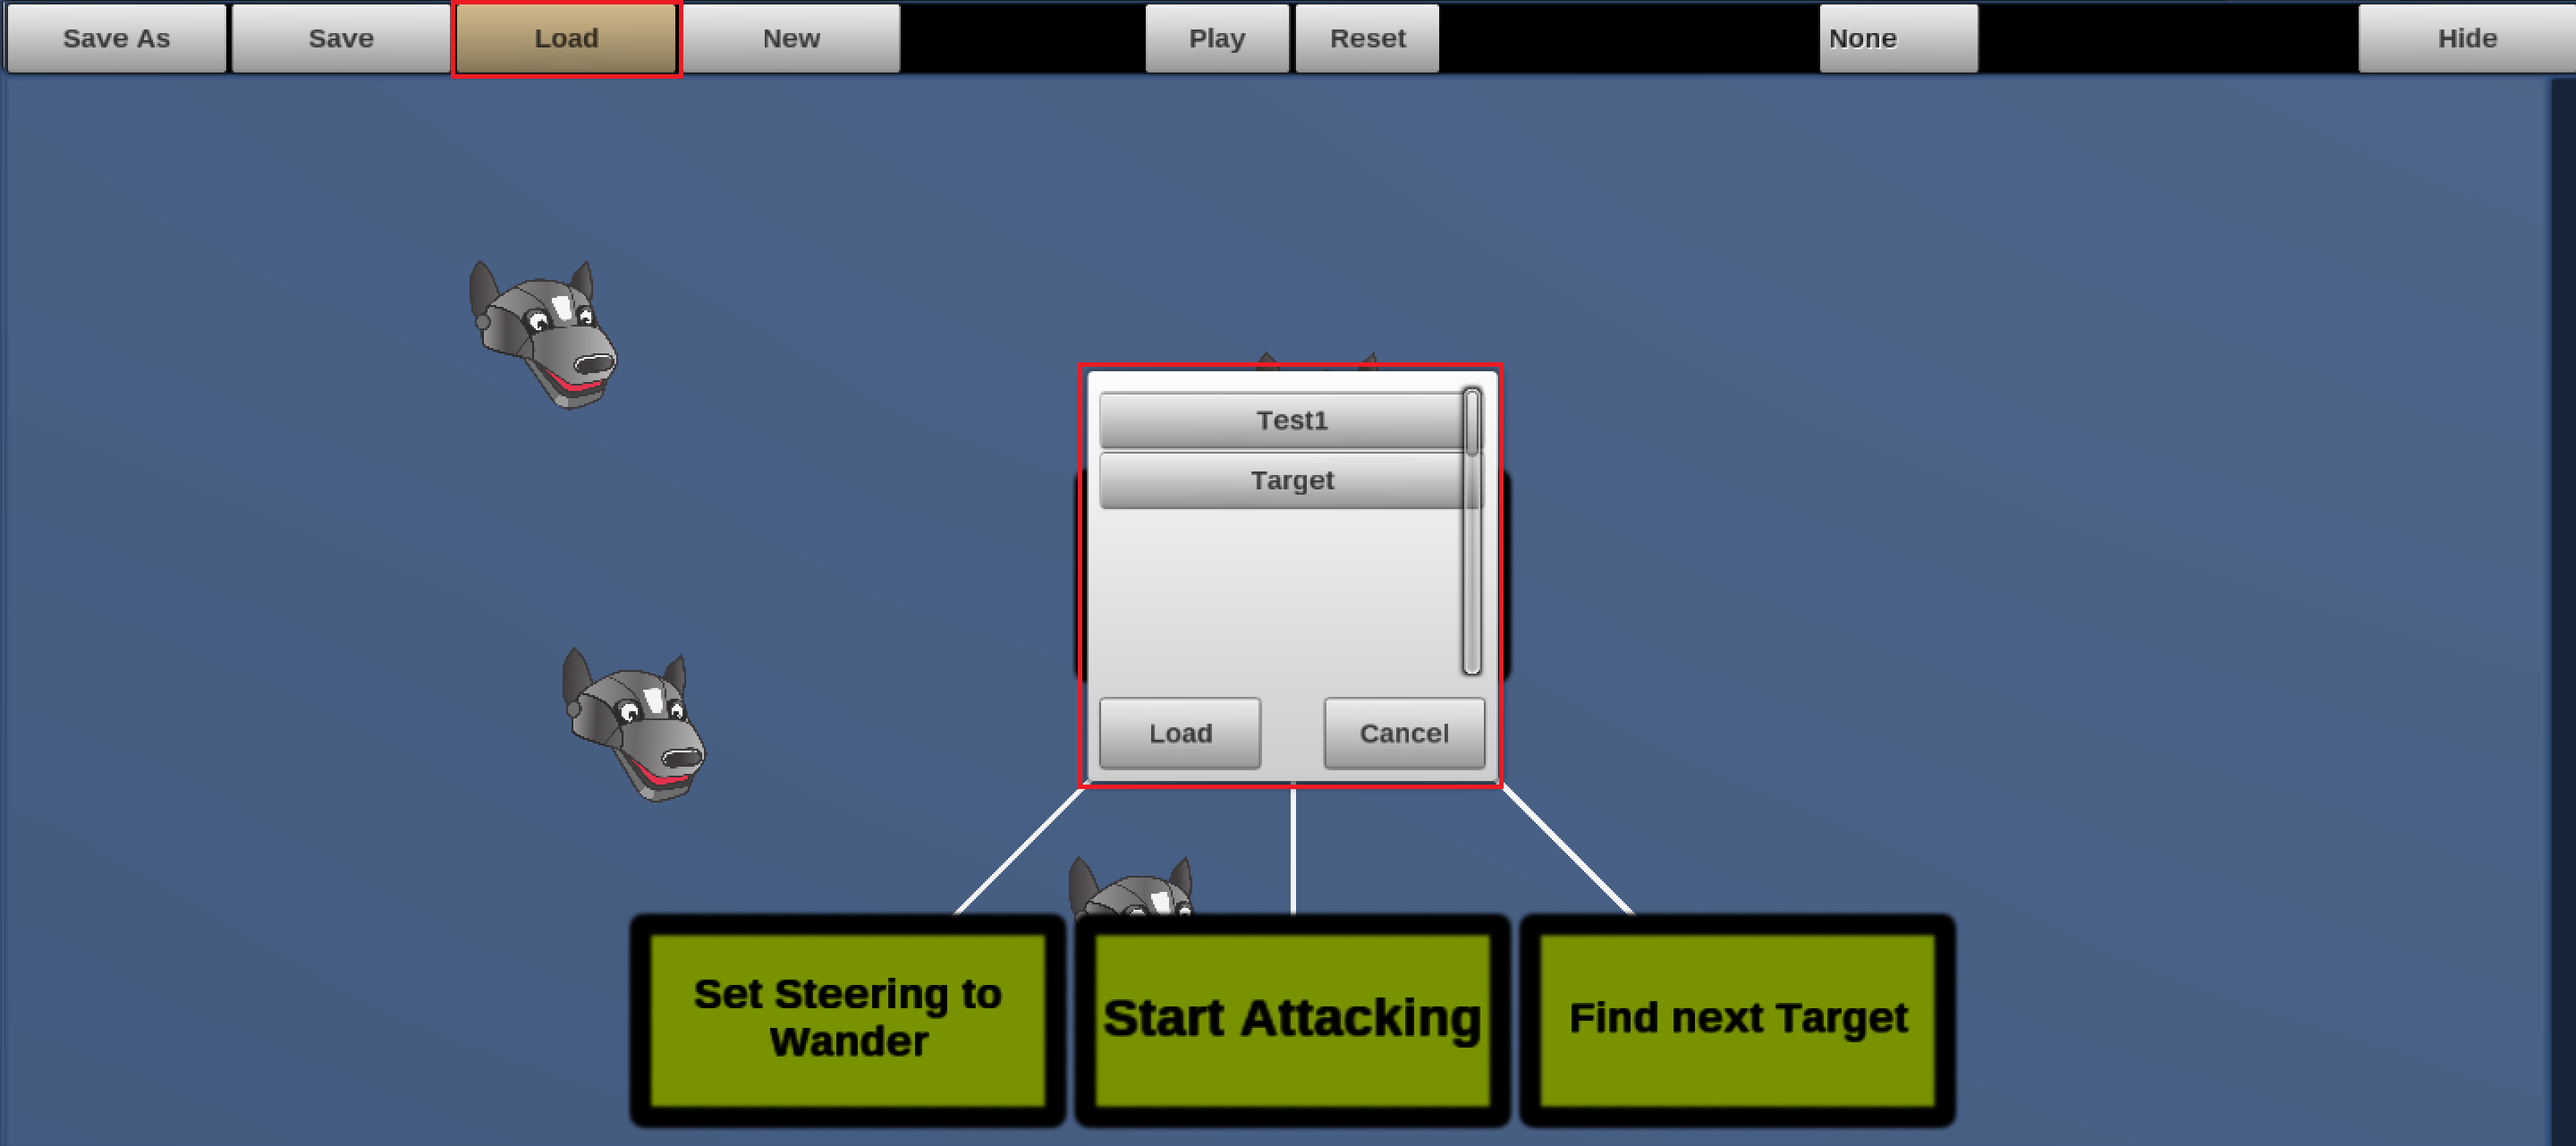
\includegraphics[width=1\textwidth]{images/KIAnleitung10_1}
	%\caption{Beziehung der BehaviourNode Klasse}
	\label{a13}
\end{figure}


\section{Ablauf des Baumes verfolgen}
Um den Ablauf eines Baumes sehen zu k�nnen, muss bereits mindestens ein Roboter mit einem Behaviour Tree ausgestattet sein. Beim Klick auf den Button mit der Aufschrift "None" �ffnet sich die Liste mit Robotern, welchen bereits ein Baum zugewiesen wurde. Sobald dort ein solcher ausgew�hlt ist, werden die anderen Funktionen des Show-Modus automatisch Deaktiviert und der zugeh�rige Baum taucht auf. Sobald das Szenario gestartet wird, werden aktuelle Pfade gr�n markiert.
\begin{figure}[h!] %[hbtp]
	\centering
		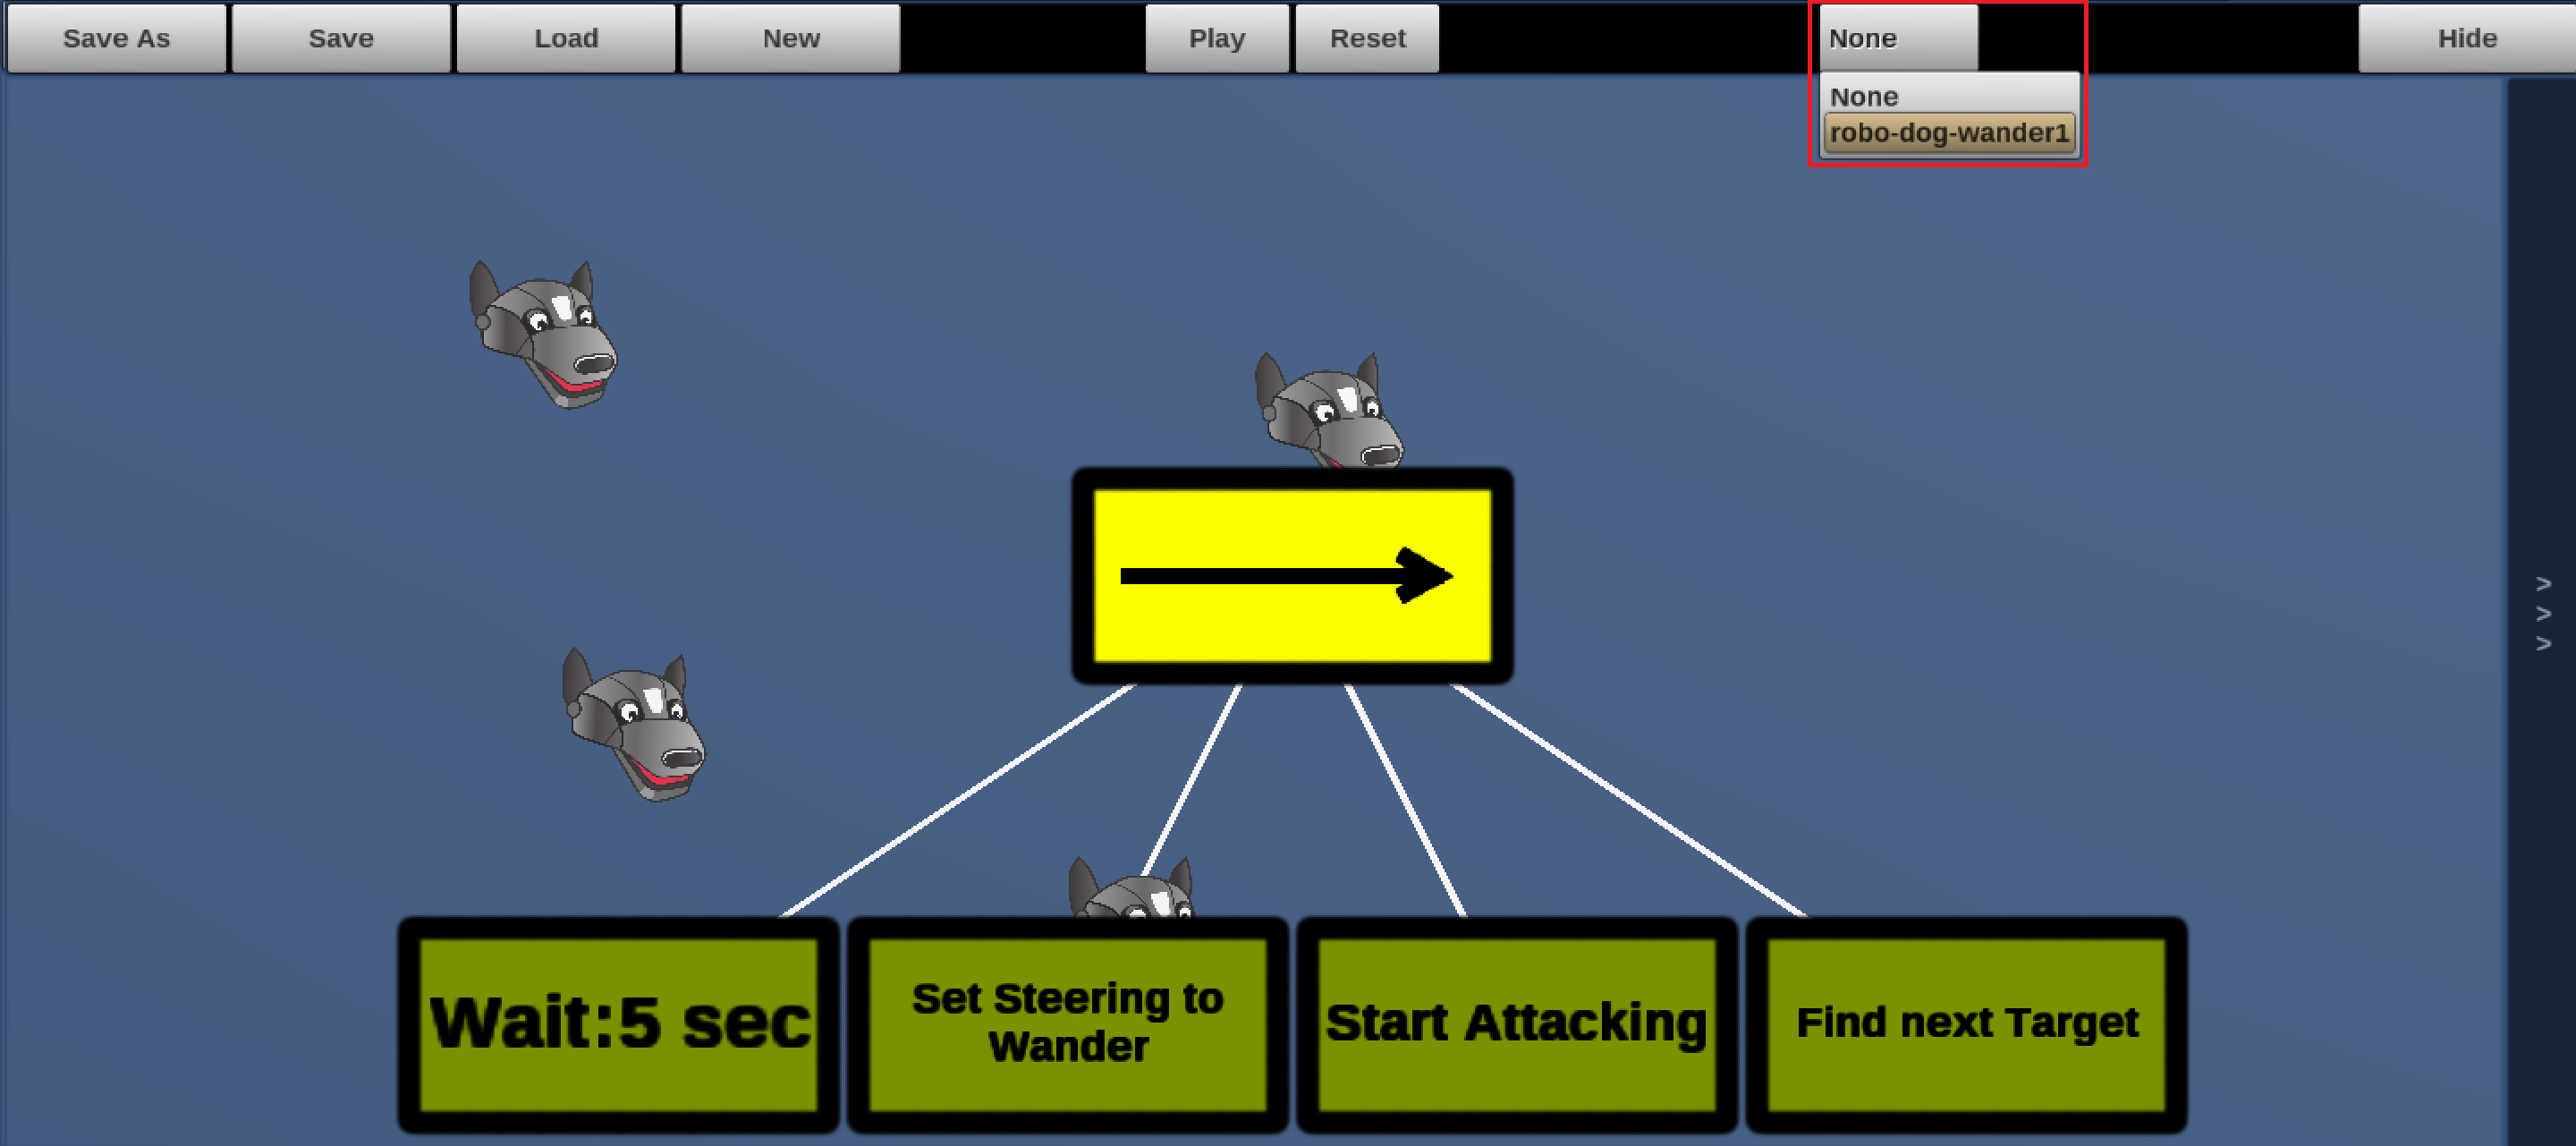
\includegraphics[width=1\textwidth]{images/KIAnleitung15_1}
	%\caption{Beziehung der BehaviourNode Klasse}
	\label{a14}
\end{figure}

\begin{figure}[h!] %[hbtp]
	\centering
		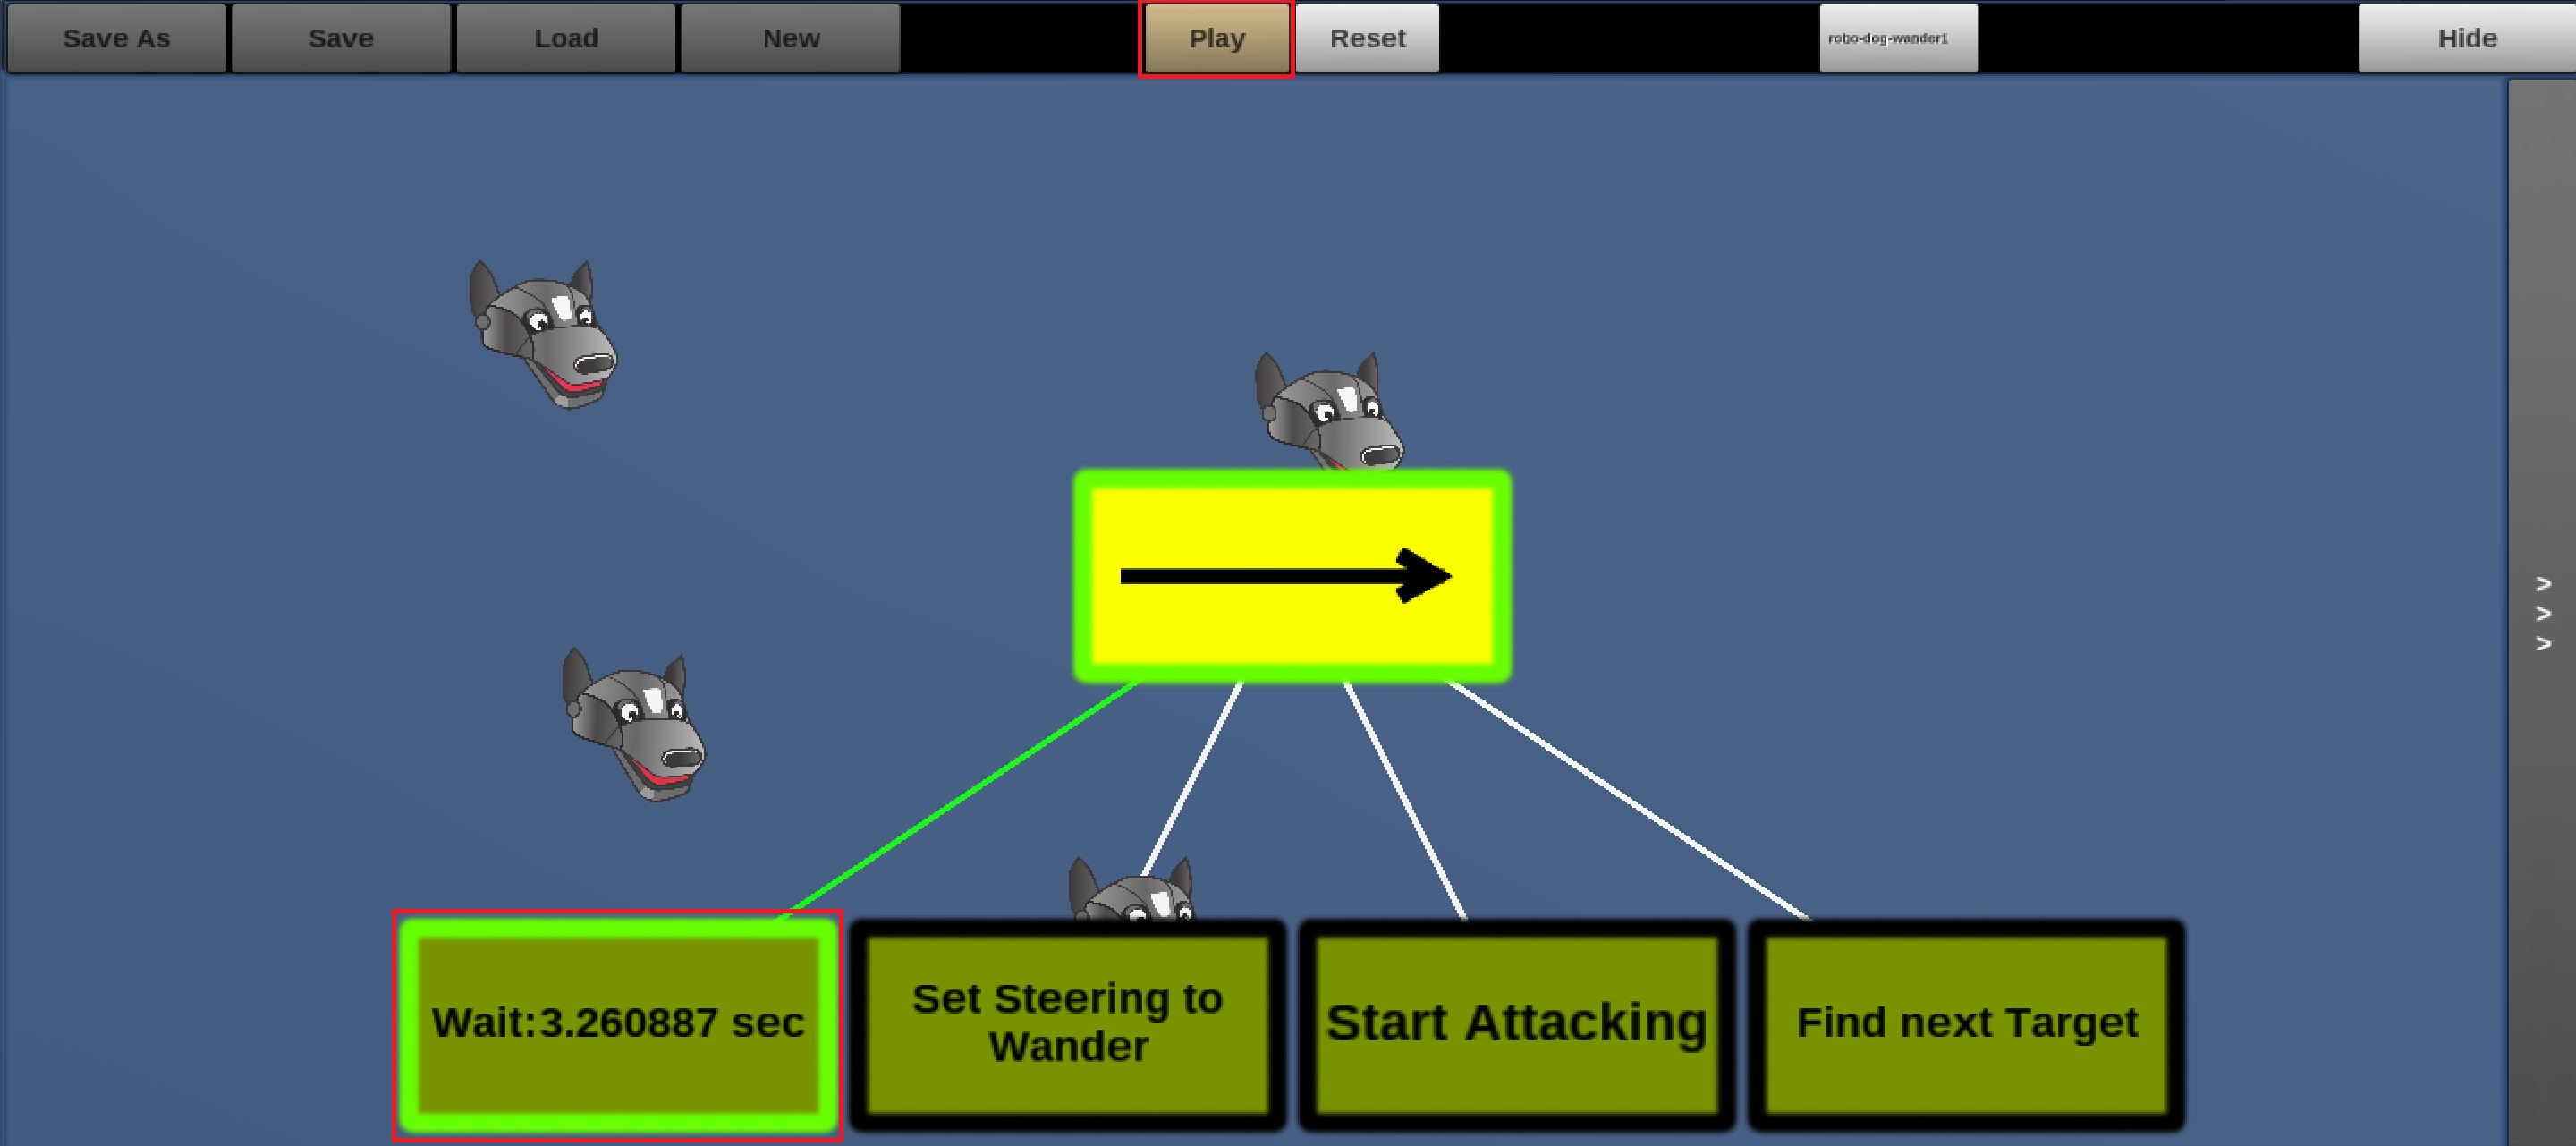
\includegraphics[width=1\textwidth]{images/KIAnleitung16_1}
	%\caption{Beziehung der BehaviourNode Klasse}
	\label{a15}
\end{figure}




Hide - Editor ist ausgeblendet
Um den Baum-Editor zu verstecken bzw. auszuschalten, wird der Hide-Button gedr�ckt.

\section{Roboter einen Baum zuweisen}
Mit dem Rechtsklick der Maus auf einen beliebigen Roboter erscheint die Liste von bereits gespeicherten B�umen. Durch die Auswahl eines Baumes wird dieser dem Roboter zugeordnet.
\begin{figure}[h!] %[hbtp]
	\centering
		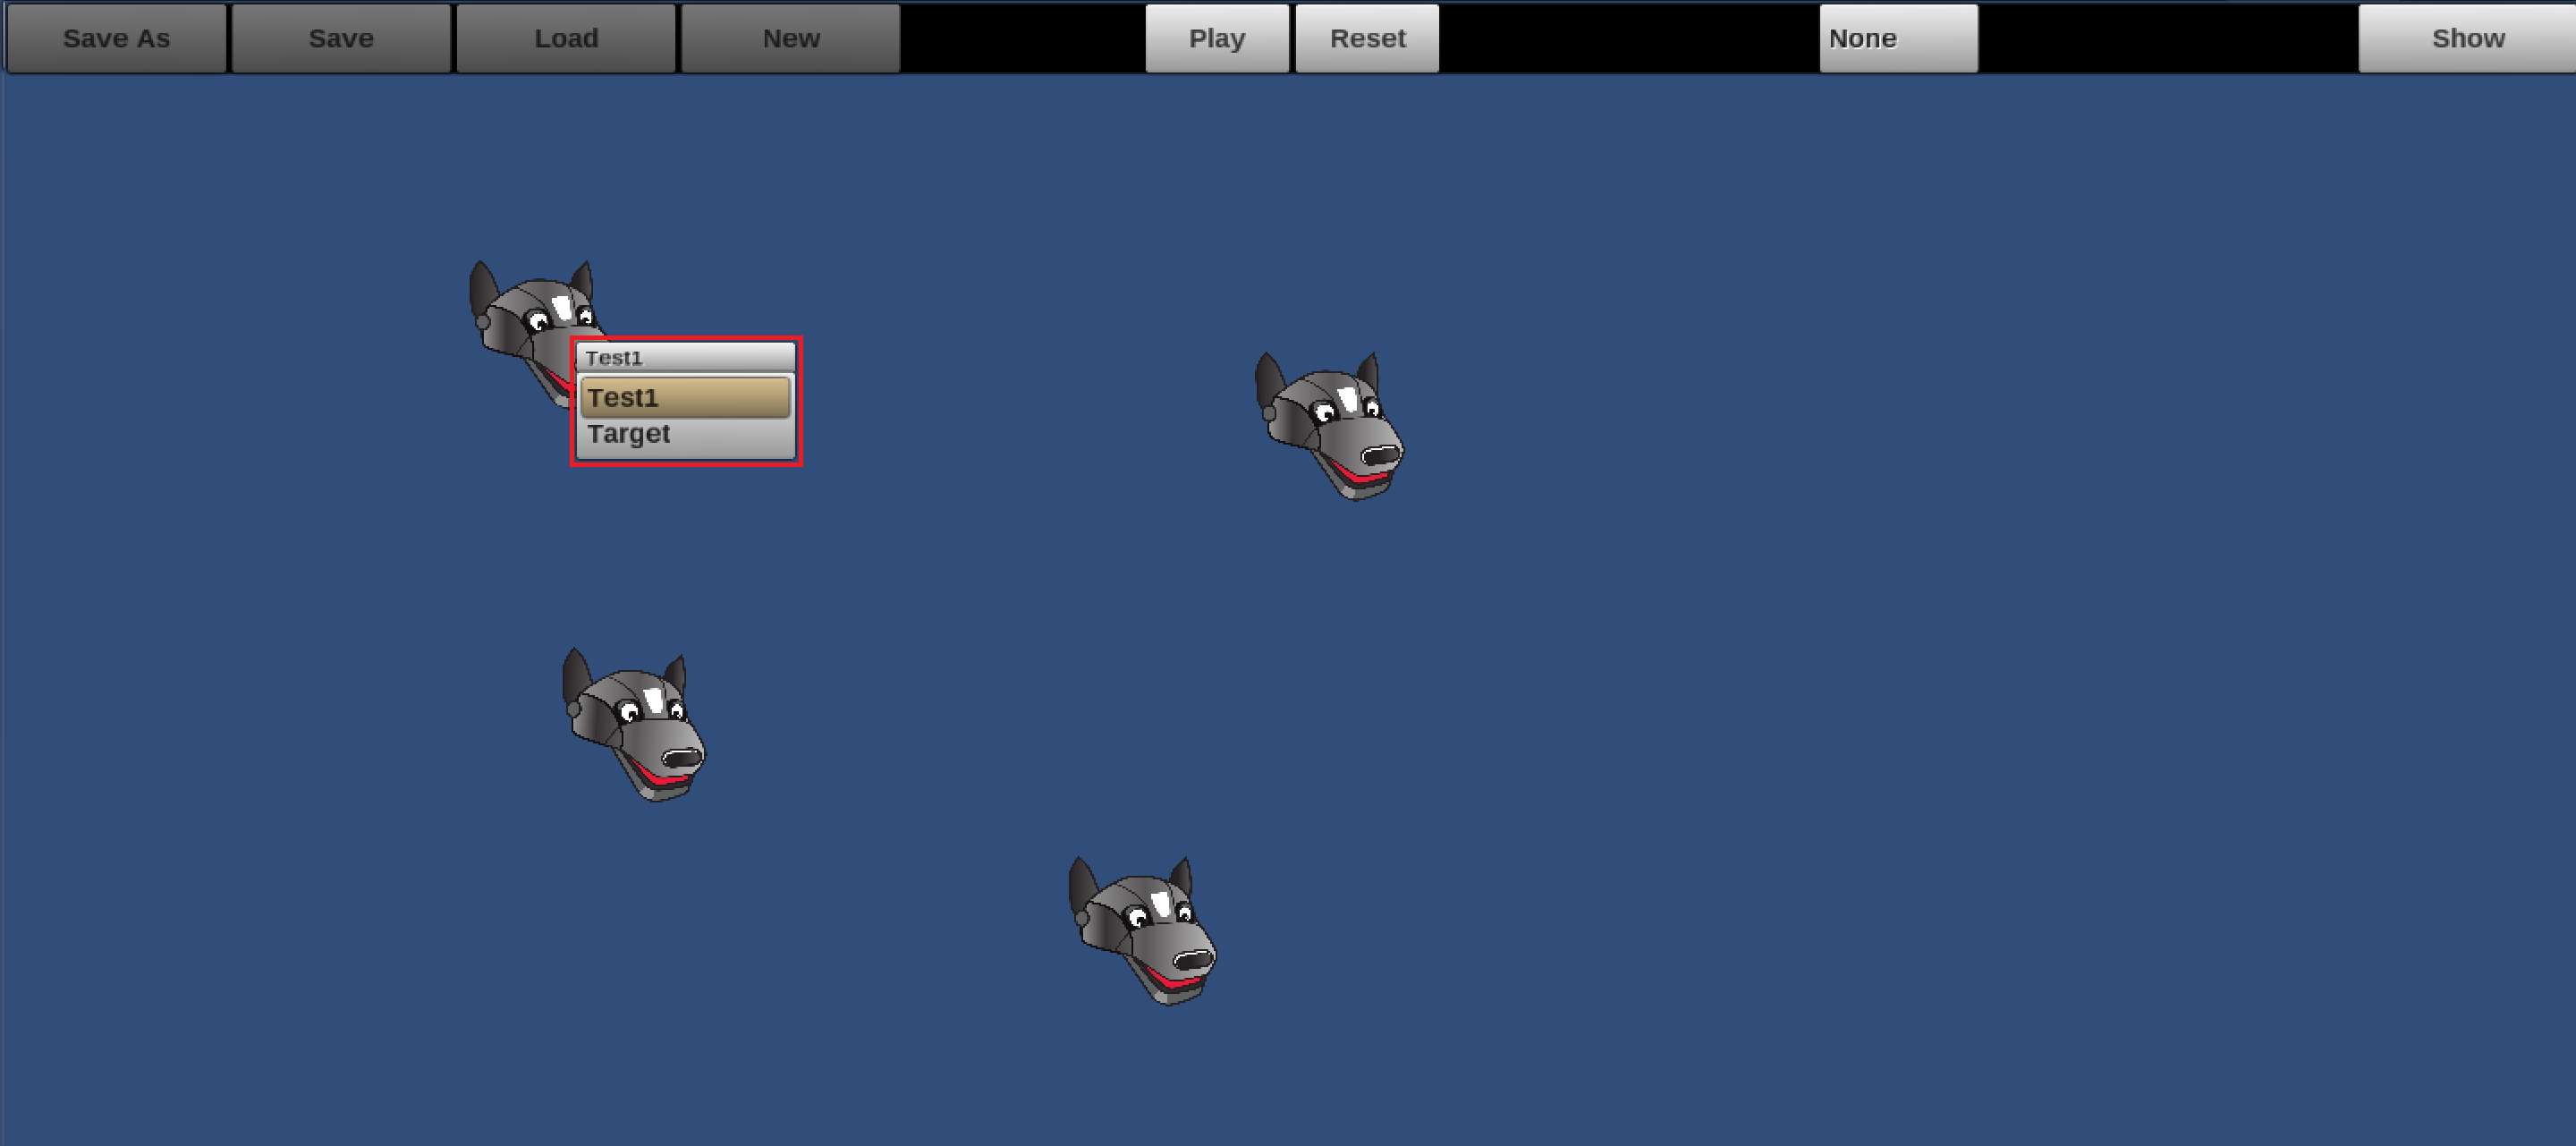
\includegraphics[width=1\textwidth]{images/KIAnleitung12_1}
	%\caption{Beziehung der BehaviourNode Klasse}
	\label{a16}
\end{figure}




Unabh�ngig von der Sichtbarkeit des Editors

\section{Szenario Starten}
Durch das Dr�cken des Start-Buttons beginnt das Szenario. Alle zugewiesenen B�ume werden automatisch aktiviert.
\begin{figure}[h!] %[hbtp]
	\centering
		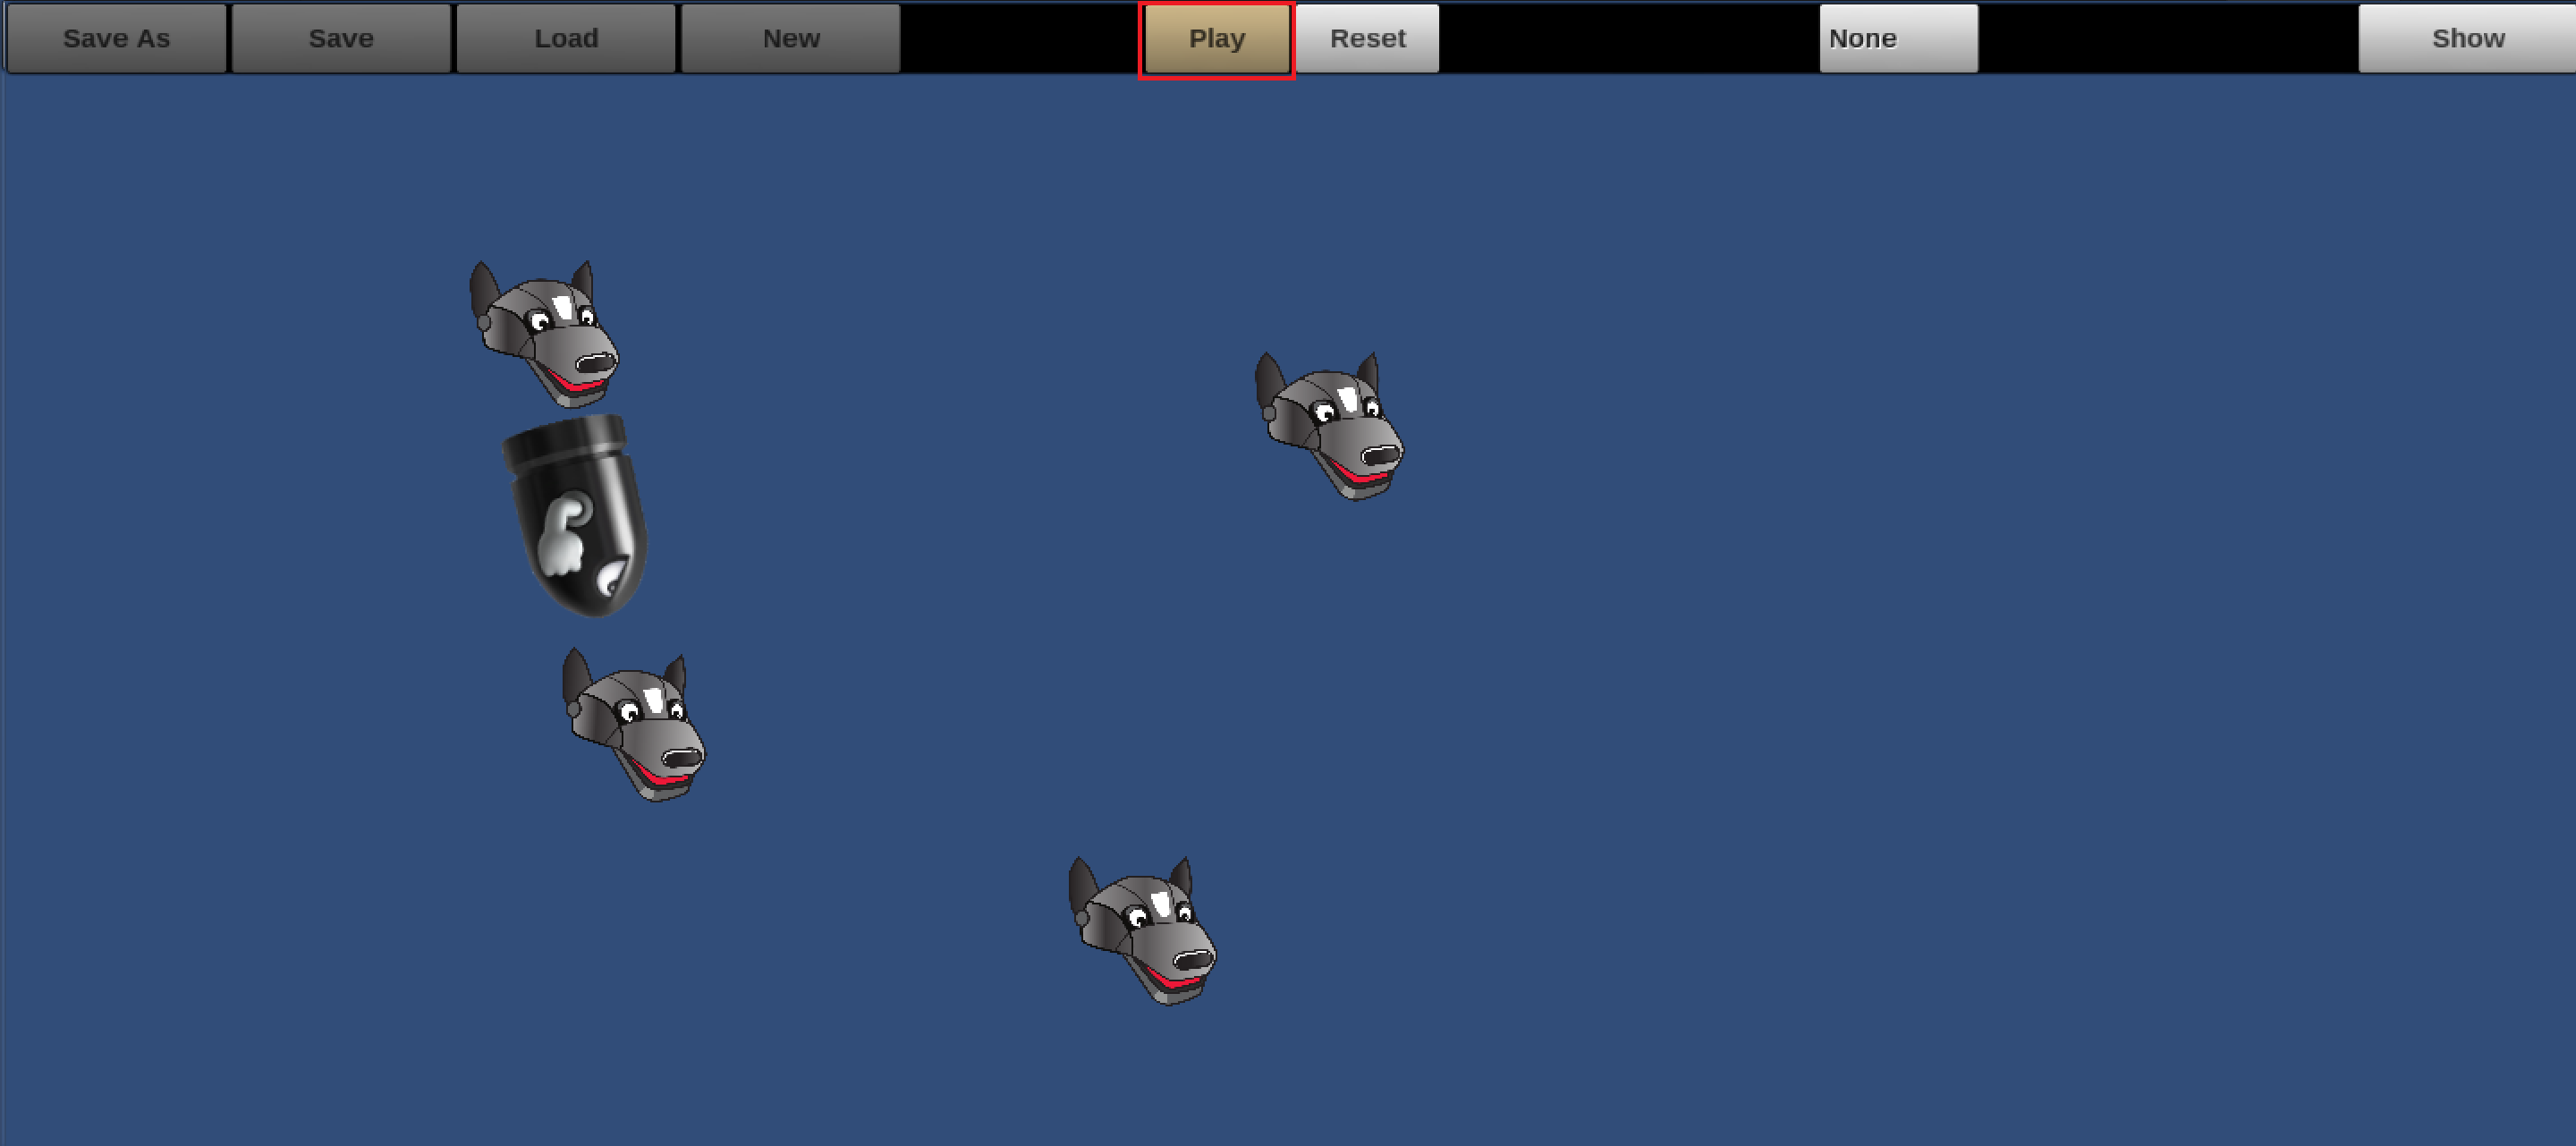
\includegraphics[width=1\textwidth]{images/KIAnleitung13_1}
	%\caption{Beziehung der BehaviourNode Klasse}
	\label{a17}
\end{figure}



\section{Szenario Zur�cksetzen}
Der Reset-Button kann jederzeit, w�hrend das Szenario l�uft, gedr�ckt werden. Alle Roboter werden auf Ihre Anfangsposition samt deren Anfangs-Attributwerten zur�ckgesetzt. Die zugewiesenen B�ume bleiben nach dem Reset erhalten.
\begin{figure}[h!] %[hbtp]
	\centering
		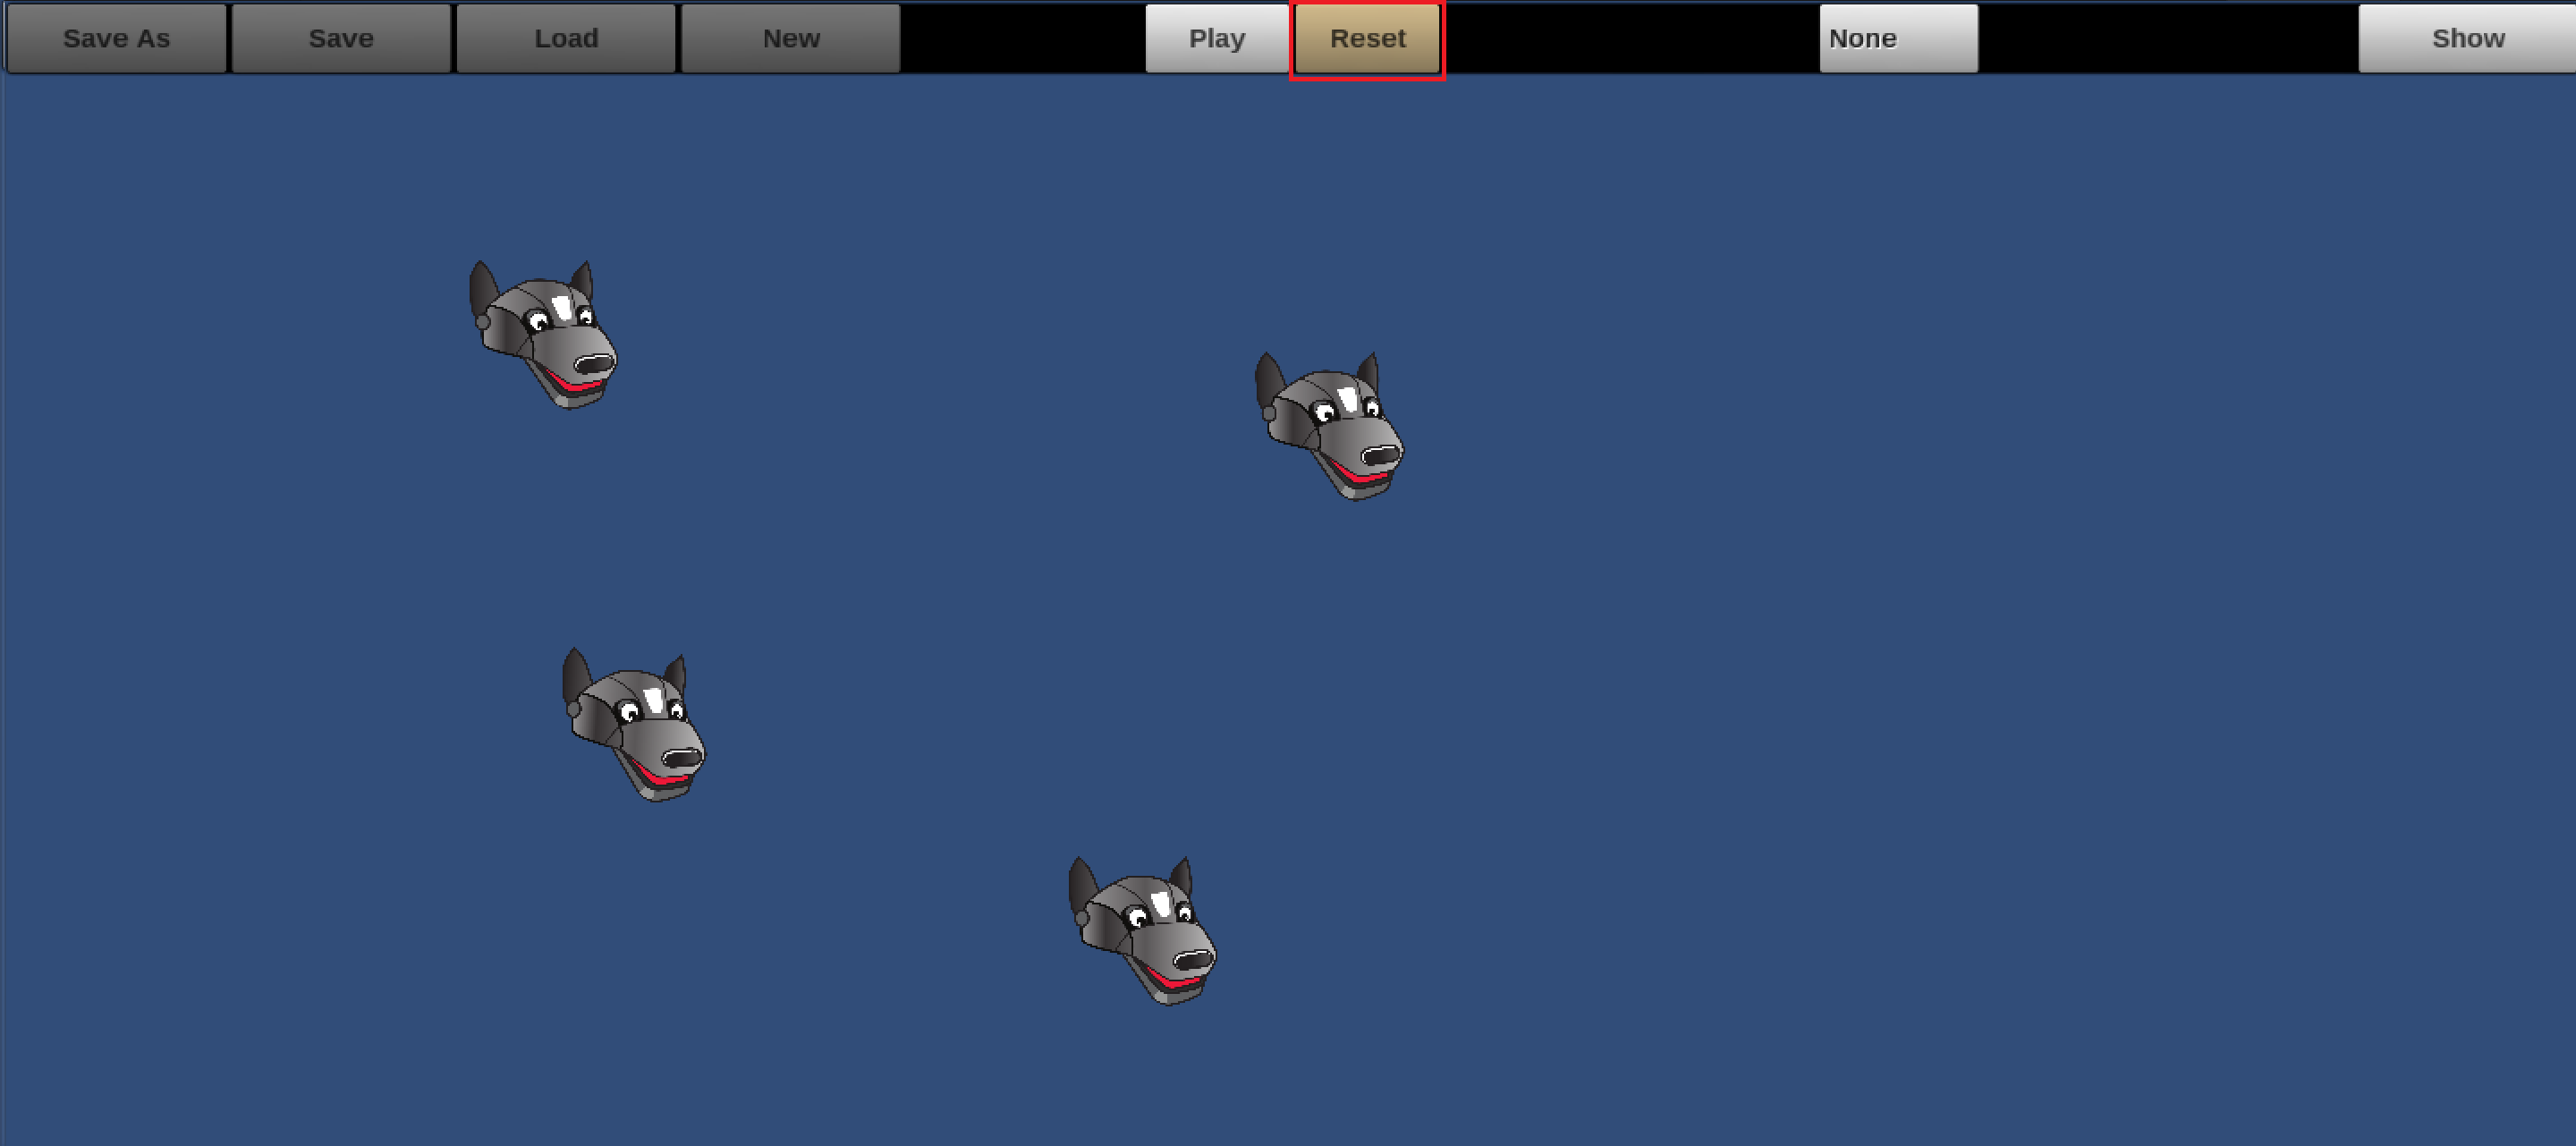
\includegraphics[width=1\textwidth]{images/KIAnleitung14_1}
	%\caption{Beziehung der BehaviourNode Klasse}
	\label{a18}
\end{figure}




% ...

%--------------------------------------------------------------------------
\backmatter                        %Anhang
%-------------------------------------------------------------------------
%Literaturverzeichnis - notwendig
%Literaturverzeichnis - notwendig
% - use bibstyle 'geralpha', 'gerplain', ...
%\bibliographystyle{gerplain}
\bibliographystyle{geralpha}
%\bibliography{literatur}     %BibTeX-File literatur.bib
%--------------------------------------------------------------------------
\printindex % Index ausdr�cken - optional
%--------------------------------------------------------------------------
% Anh�nge sind optional
%\begin{appendix}
%   \chapter{Glossar}

%geordnete tabelle, 2spaltig?
%\listofabbreviations
\abbreviation{DisASTer}		{DisASTer (Distributed Algorithms Simulation Terrain) A platform for the Implementation of Distributed Algorithms}
\abbreviation{DSM}		{		Distributed Shared Memory}
\abbreviation{AC}		{		Linearisierbarkeit (atomic consistency)}
\abbreviation{SC}		{		Sequentielle Konsistenz (sequential consistency)}
\abbreviation{WC}		{		Schwache Konsistenz (weak consistency)}
\abbreviation{RC}		{		Freigabekonsistenz (release consistency)}
   
%   \chapter{Erkl�rung der Kandidatin / des Kandidaten}

\begin{description}[$\Box$~]
\item[$\Box$] Die Arbeit habe ich selbst�ndig verfasst und keine anderen als die angegebenen Quellen- und Hilfsmittel verwendet.\\

\item[$\Box$] Die Arbeit wurde als Gruppenarbeit angefertigt. Meine eigene Leistung ist ... \\
...\\

Diesen Teil habe ich selbst�ndig verfasst und keine anderen als die angegebenen Quellen und Hilfsmittel verwendet. \\

Namen der Mitverfasser: ...

\end{description}

\vspace{2cm}

\begin{minipage}[t]{3cm}
\rule{3cm}{0.5pt}
Datum
\end{minipage}
\hfill
\begin{minipage}[t]{9cm}
\rule{9cm}{0.5pt}
Unterschrift der Kandidatin / des Kandidaten
\end{minipage} 
%\end{appendix}
\end{document}
